%Literature Survey
The first and foremost idea which considered preserving privacy while providing authentication was proposed by D. Chaum and V. Heyst in 1991 \cite{chaum1991group}. The signature model of Chaum uses group based authentication approach to implement authentication with privacy protection. Four different schemes were proposed by Chaum. Three of those schemes were undeniable signatures and a Group Manager required to communicate with every member of the group to identify the original signer. These schemes provided computational anonymity to signers. The fourth scheme was not undeniable and only provided theoretical anonymity based on selected information. Two of the proposed schemes required to calculate private key of the members beforehand that is before setting up the group. The schemes introduced by Chaum not only provided a conceptual idea of how group signature should be implemented but also provided some basic algorithms for group signature like sign, verify and open. After the introduction of group signatures, various schemes were proposed which not only improved group signature schemes of Chaum but also leads to having several additional functionalities for better application orientations. Those different schemes have varying functionality and limitations in them. The following section describes the classification of the group signature schemes based on their features.

\section{Classification of Group Signatures}\label{ClassificationGroupSignatures}
The classification of groups signature schemes can be done according to functionality present in them. All those schemes have some standard functions like group member having ability to generate a signature which can be verified in group based authentication system without revealing the identity of the signer. By using this basic principle, various types of group signatures were proposed. Some essential functionalities in those schemes are as follows.
\begin{itemize}
\item The ability of the schemes to generate a private key of a member after creation/setup of the group.
\item The capability to produce verifiable proof that a given signature can be linked to one and only one signer.
\item The ability of distribution of power possessed by Group Manager into multiple entities like separate entity for opening signature rather than Group Manager alone.
\end{itemize}

The classification of group signature in the section is based on functional properties present in the schemes. It also provides a high-level overview of algorithms present in group signature schemes. The classification given below includes almost all the major group signature scheme which existed till now.
\subsection{Static Group Signatures}
The static group signature scheme\index{static group signature scheme} is very primitive and straightforward signature scheme among all the group signature schemes. In static group signature scheme, the number of group members is fixed and decided at the beginning of the group and before the setup of the group. The private keys of the group members were computed before setup of the group and cannot be calculated after the setup. Therefore only fixed members are allowed in the static group signature scheme. 

The Group Manager in these schemes is almost always a single entity, bearing the responsibilities of computing the private keys of the group members, distribution of these private keys to the members and linking signature to their original signer. The formal definition of the static group signature is as follows. The definition and description of algorithms are based on the model of static group signature proposed by Bellare, Micciancio, and Warinschi \cite{bellare2003foundations}.
\nomenclature{gpk}{group public key}
\nomenclature{gsk}{group private key}
\nomenclature{mpk}{member's private key}
\begin{definition}[Static group signature scheme] A static group signature scheme consists of following four algorithms.\\
\textbf{SetUp:} The randomized \texttt{SetUp} algorithm takes input security parameters $(1^k, n)$ where $k\in \mathbb{N}$  and $n$ as the number of group members $n\in \mathbb{N}$ and generates a tuple $(gpk, gsk, mpk)$ where $gpk$ is group public key, $gsk$ is group private key, $mpk$ is member's private key is an array with $mpk\lbrack i \rbrack$ is the private key of the member $i$.\\	
\textbf{Sign:} The randomized algorithm \texttt{Sign} produces a signature $S$ for a message by taking input $(mpk, M)$ where $mpk$ is member private key and $M$ is the message.\\
\textbf{Verify:} The deterministic signature \texttt{Verify} algorithm determines the validity of a signature on a message $M$ by taking input $(gpk, M, S)$ where $gpk$ is group public key, $M$ is the message, $S$ is signature and returning \texttt{true} for valid and \texttt{false} for invalid signature.\\
\textbf{Open:} The deterministic algorithm \texttt{Open} returns $mpk$ that is members private key by taking input $(gsk, S)$ where $gsk$ is group private key and $S$ is the signature for a message. It is required that the validity of the signature must be true by \texttt{Verify} algorithm to return correct $mpk$.
\end{definition}

\begin{figure}[h]
    \centering
    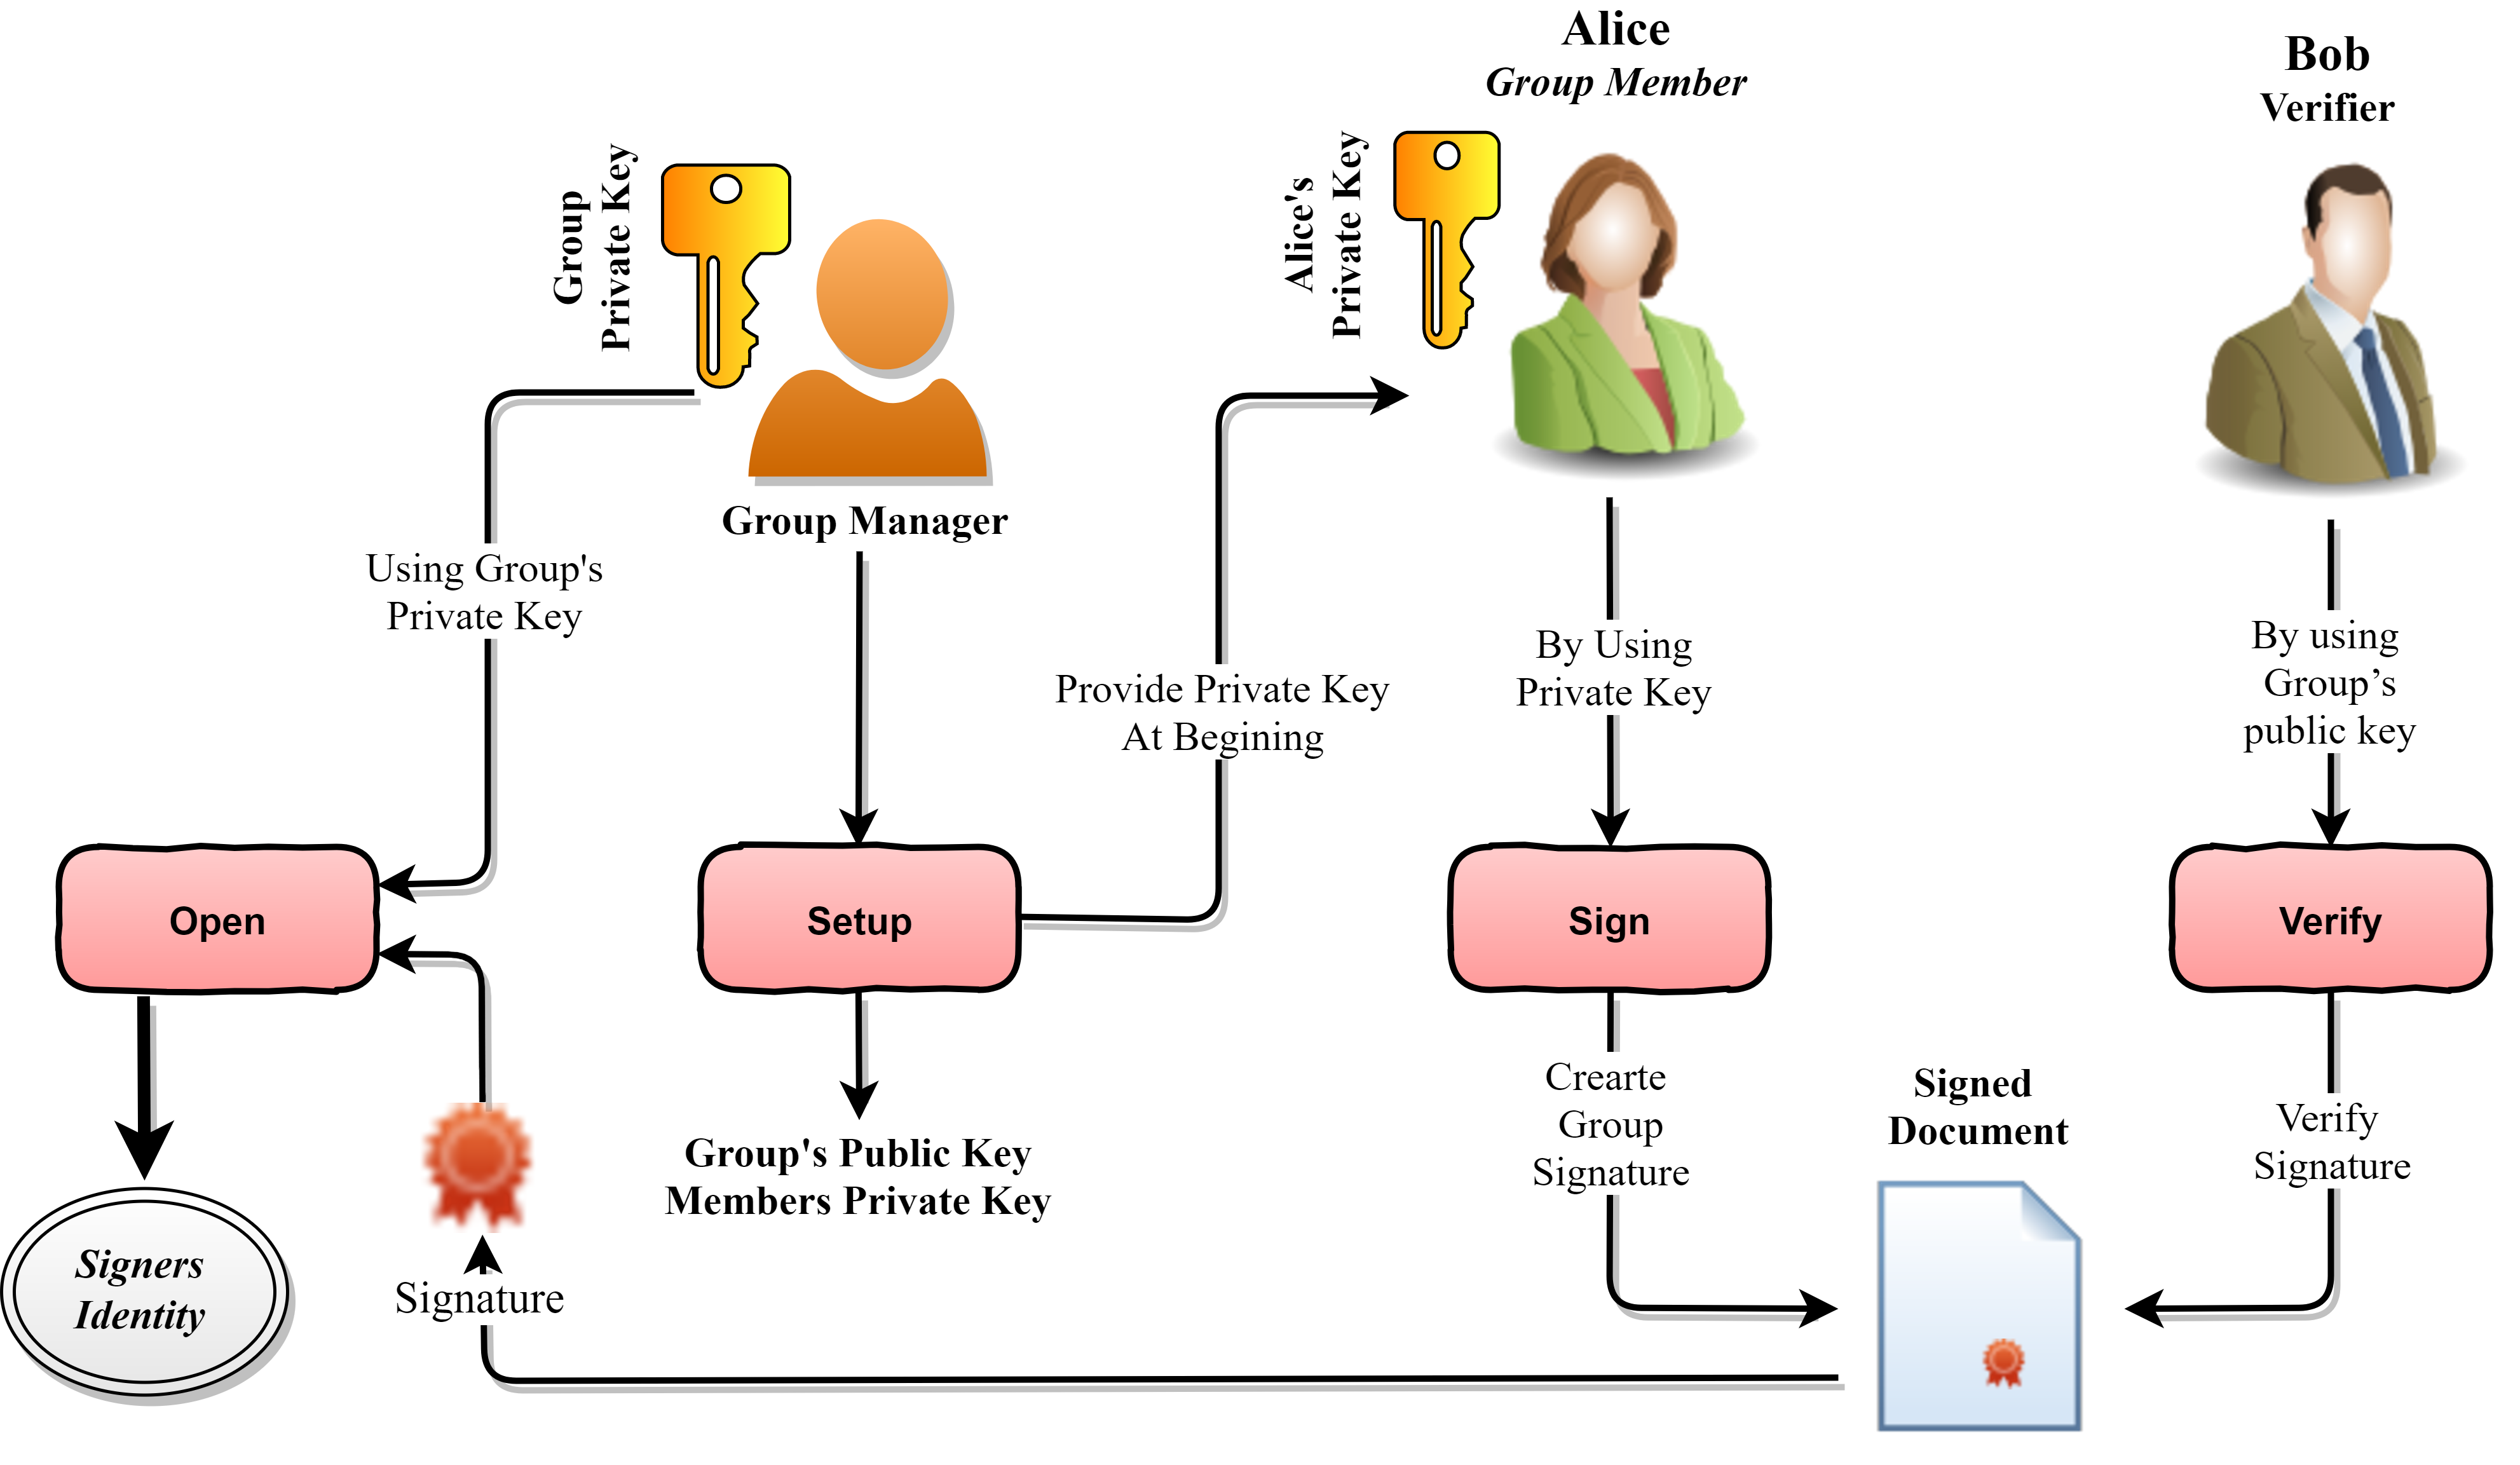
\includegraphics[width=\textwidth]{StaticGroupSignature}
    \caption{Static Group Signatures Scheme}
    \label{fig:Static Group Signatures Scheme}
\end{figure}

The figure \ref{fig:Static Group Signatures Scheme} describes the procedure of static group signature scheme. First, the Group Manager generate Group Private key, Group Public key and private keys of all the members. Group Manager then distributes the private keys of members to them securely. Once the members get their private key, they can generate the signature for any message. Alice as a group member receives her private key from Group Manager. To sign a message, Alice uses her private key to produce the signature for the message and the message along with the signature is transmitted to Bob, who is a verifier via an insecure channel. To verify the signature of the message, Bob executes Verify algorithm which determines the validity of the signature but does not disclose any information about signer, in this case, Alice. To link the signature to its original signer, the Group Manager executes the Open algorithm which returns the identity of the signer, in this case, the identity of Alice. 

Note that although static group signature schemes have a fixed number of members, these schemes can offer the functionality of revocation of the members which allows removing members from the group (but can not add any new members).

\subsection{Dynamic Group Signatures}\label{sub:Dynamic Group Signatures}
The static group signatures have the limitation of not only fixed number of members but also the requirement of deciding their number at the commencement of the group. Many applications of group signature are not able to be implemented because of such limitations of static group signatures. Those applications require the ability of addition of members at any time after commencement the group. The dynamic group signature scheme does not have limitations of fixed members determined at the beginning of group like static group signatures.

In the dynamic group signature scheme\index{dynamic group signature scheme}, the Group Manager can add any number of members at any time after commencement of the group. It implies that the private key of a new member can be generated after the creation of the group. The dynamic group signature scheme has an additional join protocol in extension to the four protocols in static group signatures. The join protocol is a protocol between Group Manager and a user who wishes to become a member of the group. To implement this dynamic member join protocol, the remaining algorithm in group signature, especially the setup algorithm required to be altered.

Similar to static group signatures, some dynamic group signature may offer the functionality of revocation of the group members. The revoked members cannot produce a valid group signature. These schemes have a true dynamic-ness in them, as they can add and remove any member of the group at any time. The following section provides the definition of dynamic group signature scheme and description of the algorithms in it.

\begin{definition}[Dynamic group signature scheme]A dynamic group signature scheme consist of following five algorithm/protocols.\\
\textbf{SetUp:} The randomized \texttt{SetUp} algorithm takes an input of security parameter $1^k$ where $k\in \mathbb{N}$ and generates a tuple $(gpk, gsk, List)$ where $gpk$ is group public key, $gsk$ is group private key, $List$ is a list of members of the group. The $List$ is empty at the commencement of the group.\\
\textbf{Join:} The randomized \texttt{Join} algorithm is a protocol between Group Manager and a user which takes an input of $gsk$ from Group Manager and produce $mpk$ which is members private key for the user making him a valid group member. It also adds the credentials of the user into the list like his $mpk$.\\
\textbf{Sign:} The randomized algorithm \texttt{Sign} produces a signature $S$ for a message by taking input $(mpk, M)$ where $mpk$ is member private key and $M$ is the message.\\
\textbf{Verify:} The deterministic signature \texttt{Verify} algorithm determines the validity of a signature on a message $M$ by taking input $(gpk, M, S)$ where $gpk$ is group public key, $M$ is the message, $S$ is signature and returning \texttt{true} for valid and \texttt{false} for invalid signature.\\
\textbf{Open:} The deterministic algorithm \texttt{Open} returns $mpk$ that is members private key by taking input $(gsk, S)$ where $gsk$ is group private key and $S$ is the signature for a message. It is required that the validity of the signature must be true by \texttt{Verify} algorithm to return correct $mpk$.
\end{definition}
\begin{figure}[h]
    \centering
    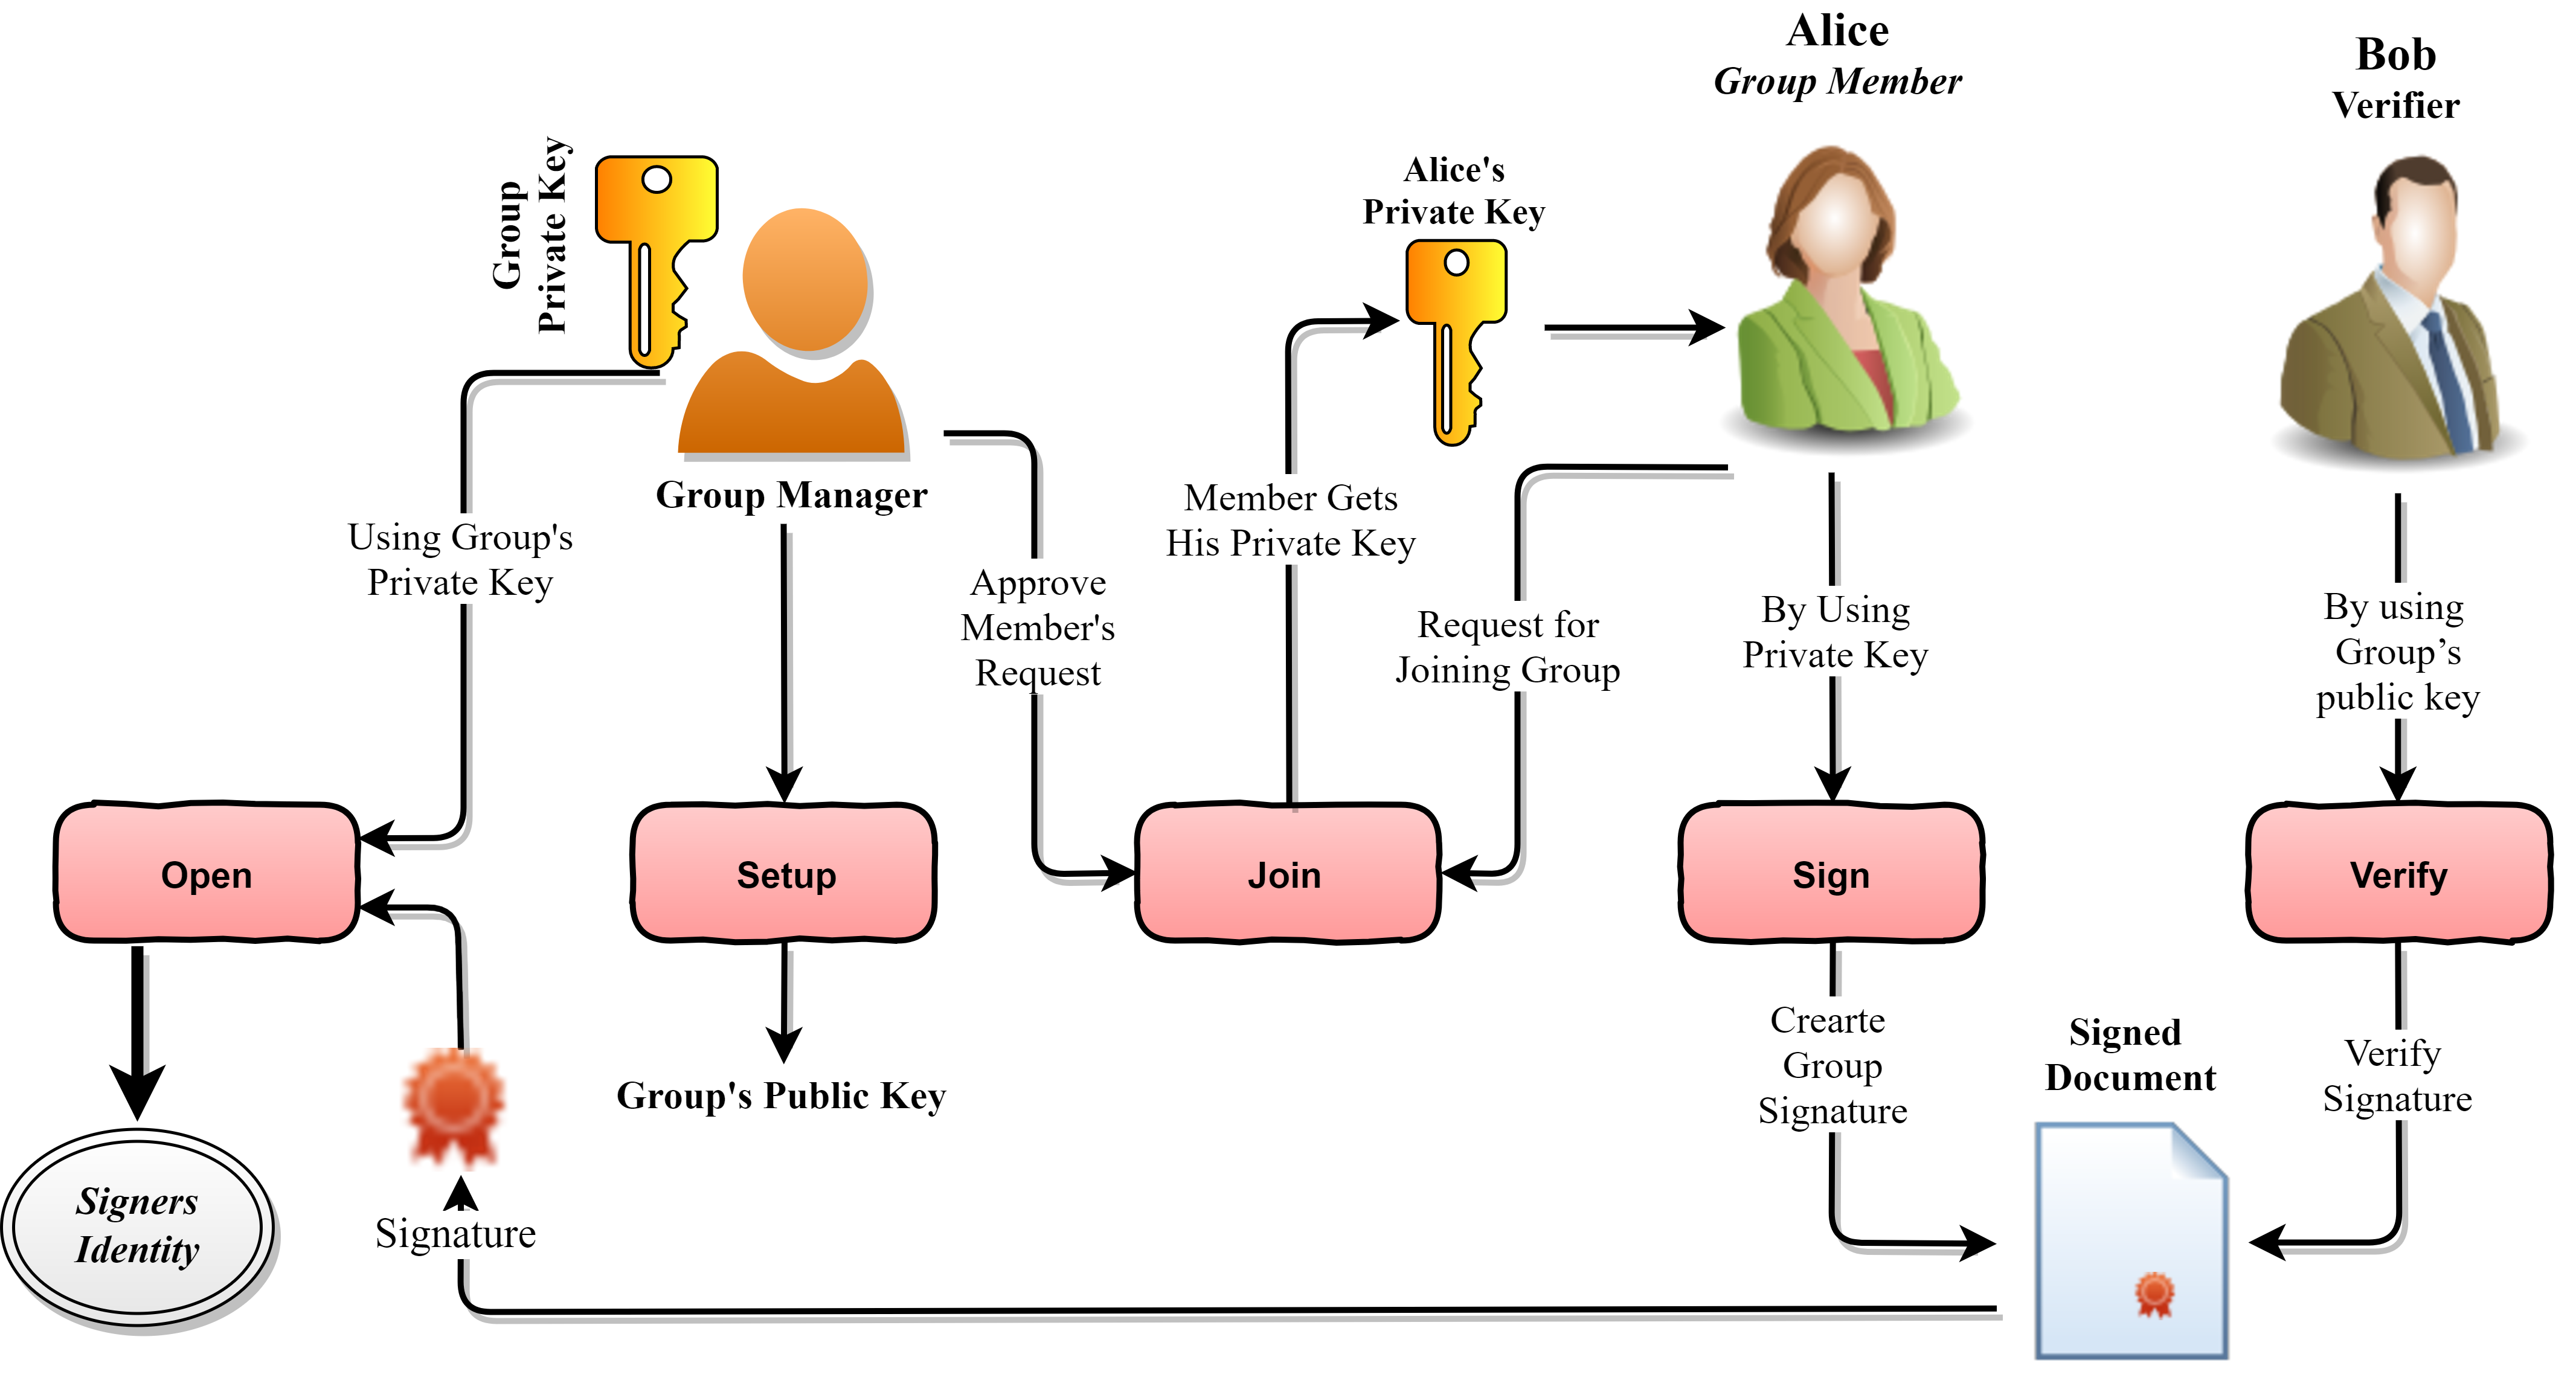
\includegraphics[width=\textwidth]{DynamicGroupSignature}
    \caption{Dynamic Group Signatures Scheme}
    \label{fig:Dynamic Group Signatures Scheme}
\end{figure}
The figure \ref{fig:Dynamic Group Signatures Scheme} describes the procedure of dynamic group signature scheme. Initially the Group Manager setup the group creating his private key and groups public key. When Alice as a user wants to join the group, she requests to the Group Manager by using the join protocol. The Group Manager then approves the request sent by Alice and the join algorithm provides a private key to the member, in this case, Alice and add his credential into the database. The Group Manager may or may not know the $mpk$ of member depending on the scheme, but as a trusted authority, Group Manager is supposed to be having knowledge of $mpk$ of all the members. After becoming the member of the group by getting her private key, Alice as a group member is now able to produce group signature by using sign algorithm for any message. After signing a message, Alice transmits the signed message along with the signature to Bob, who is a potential verifier via an insecure channel. To verify the signature of the message Bob executes the verify algorithm which determines the validity of the signature. Note that during the transmission of the message Alice not needed to show her name as sender or signer. It is also possible to publish the message to the intended receiver anonymously.

Note that although the dynamic group signature does not have a fixed number of members, theoretically the scheme always have an upper bound $n$ which denotes the maximum number of possible members in a group. It should be taken care that the upper bound $n$ should be large enough so that all the possible number of members can join the group without approaching its limit.
\subsection{Group Signature Schemes with Verifiable Opening}
\index{group signature schemes with verifiable opening}The group signatures have a unique property of not only preserving the privacy of the signer but also provide the power of traceability to a trusted authority. The trusted authority like Group Manager can associate a signature to its original signer by using his private key. But the opening of the signature is usually fall-back mechanism and infrequently used. The opening of the signature usually follows subsequent actions on the signer like his revocation form the group. In such cases, the actions of the opening entity like Group Manager are required to be completely selfless, and any member is not being accused falsely by the Group Manager. The trust level of the Group Manager needs not to be required of a very high level when there can be a mechanism of publicly verifiable proof. The group signature with publicly verifiable opening provides the same mechanism. 

In these group signature schemes when the opening of the signature is performed, the Group Manager not only provide the identification of the signer but also provide a publicly verifiable proof that any user can verify and conclude that the Group Manager is not falsely accusing any member, for a signature. The proof provided by Group Manager mathematically proves that the identity of the signer is in did the one whose signature Group Manager claim it to be. The functionality of the publicly verifiable proof can be implemented by improving or modifying the opening algorithm in group signature scheme. This modified opening algorithm provides a publicly verifiable proof along with the identification of the signer. An additional algorithm is required for judgment or verification of the proof given by the opening algorithm, which determines the truthfulness of the proof. This Judge algorithm should always be publicly accessible so that anyone can verify the sincerity of the proof. Following section provide the definition of the group signature scheme with variable opening and description of the algorithms in it.

\begin{definition}[Group Signature Schemes with Verifiable Opening] A group signature scheme with a variable opening is a static or dynamic group signature scheme with an improved opening algorithm and an additional judge algorithm for public verification of result of the opening algorithm.\\
\textbf{Open algorithm:} The deterministic algorithm \texttt{Open} produces output of pair (signer's identity $i$ and proof $\mathbb{T}$) it by taking input of $(gsk, S)$.\\
\textbf{Judge algorithm:} The deterministic algorithm \texttt{Judge} produces a result of validity of the proof, generated by the \texttt{Open} algorithm. That is \texttt{true} for valid and \texttt{false} for invalid proof, after taking the input of $(gpk, M, S, i, \mathbb{T})$ where $i$ is the identity of the signer and $\mathbb{T}$ is proof produced by the \texttt{Open} algorithm.
\end{definition}
\begin{figure}[h]
    \centering
    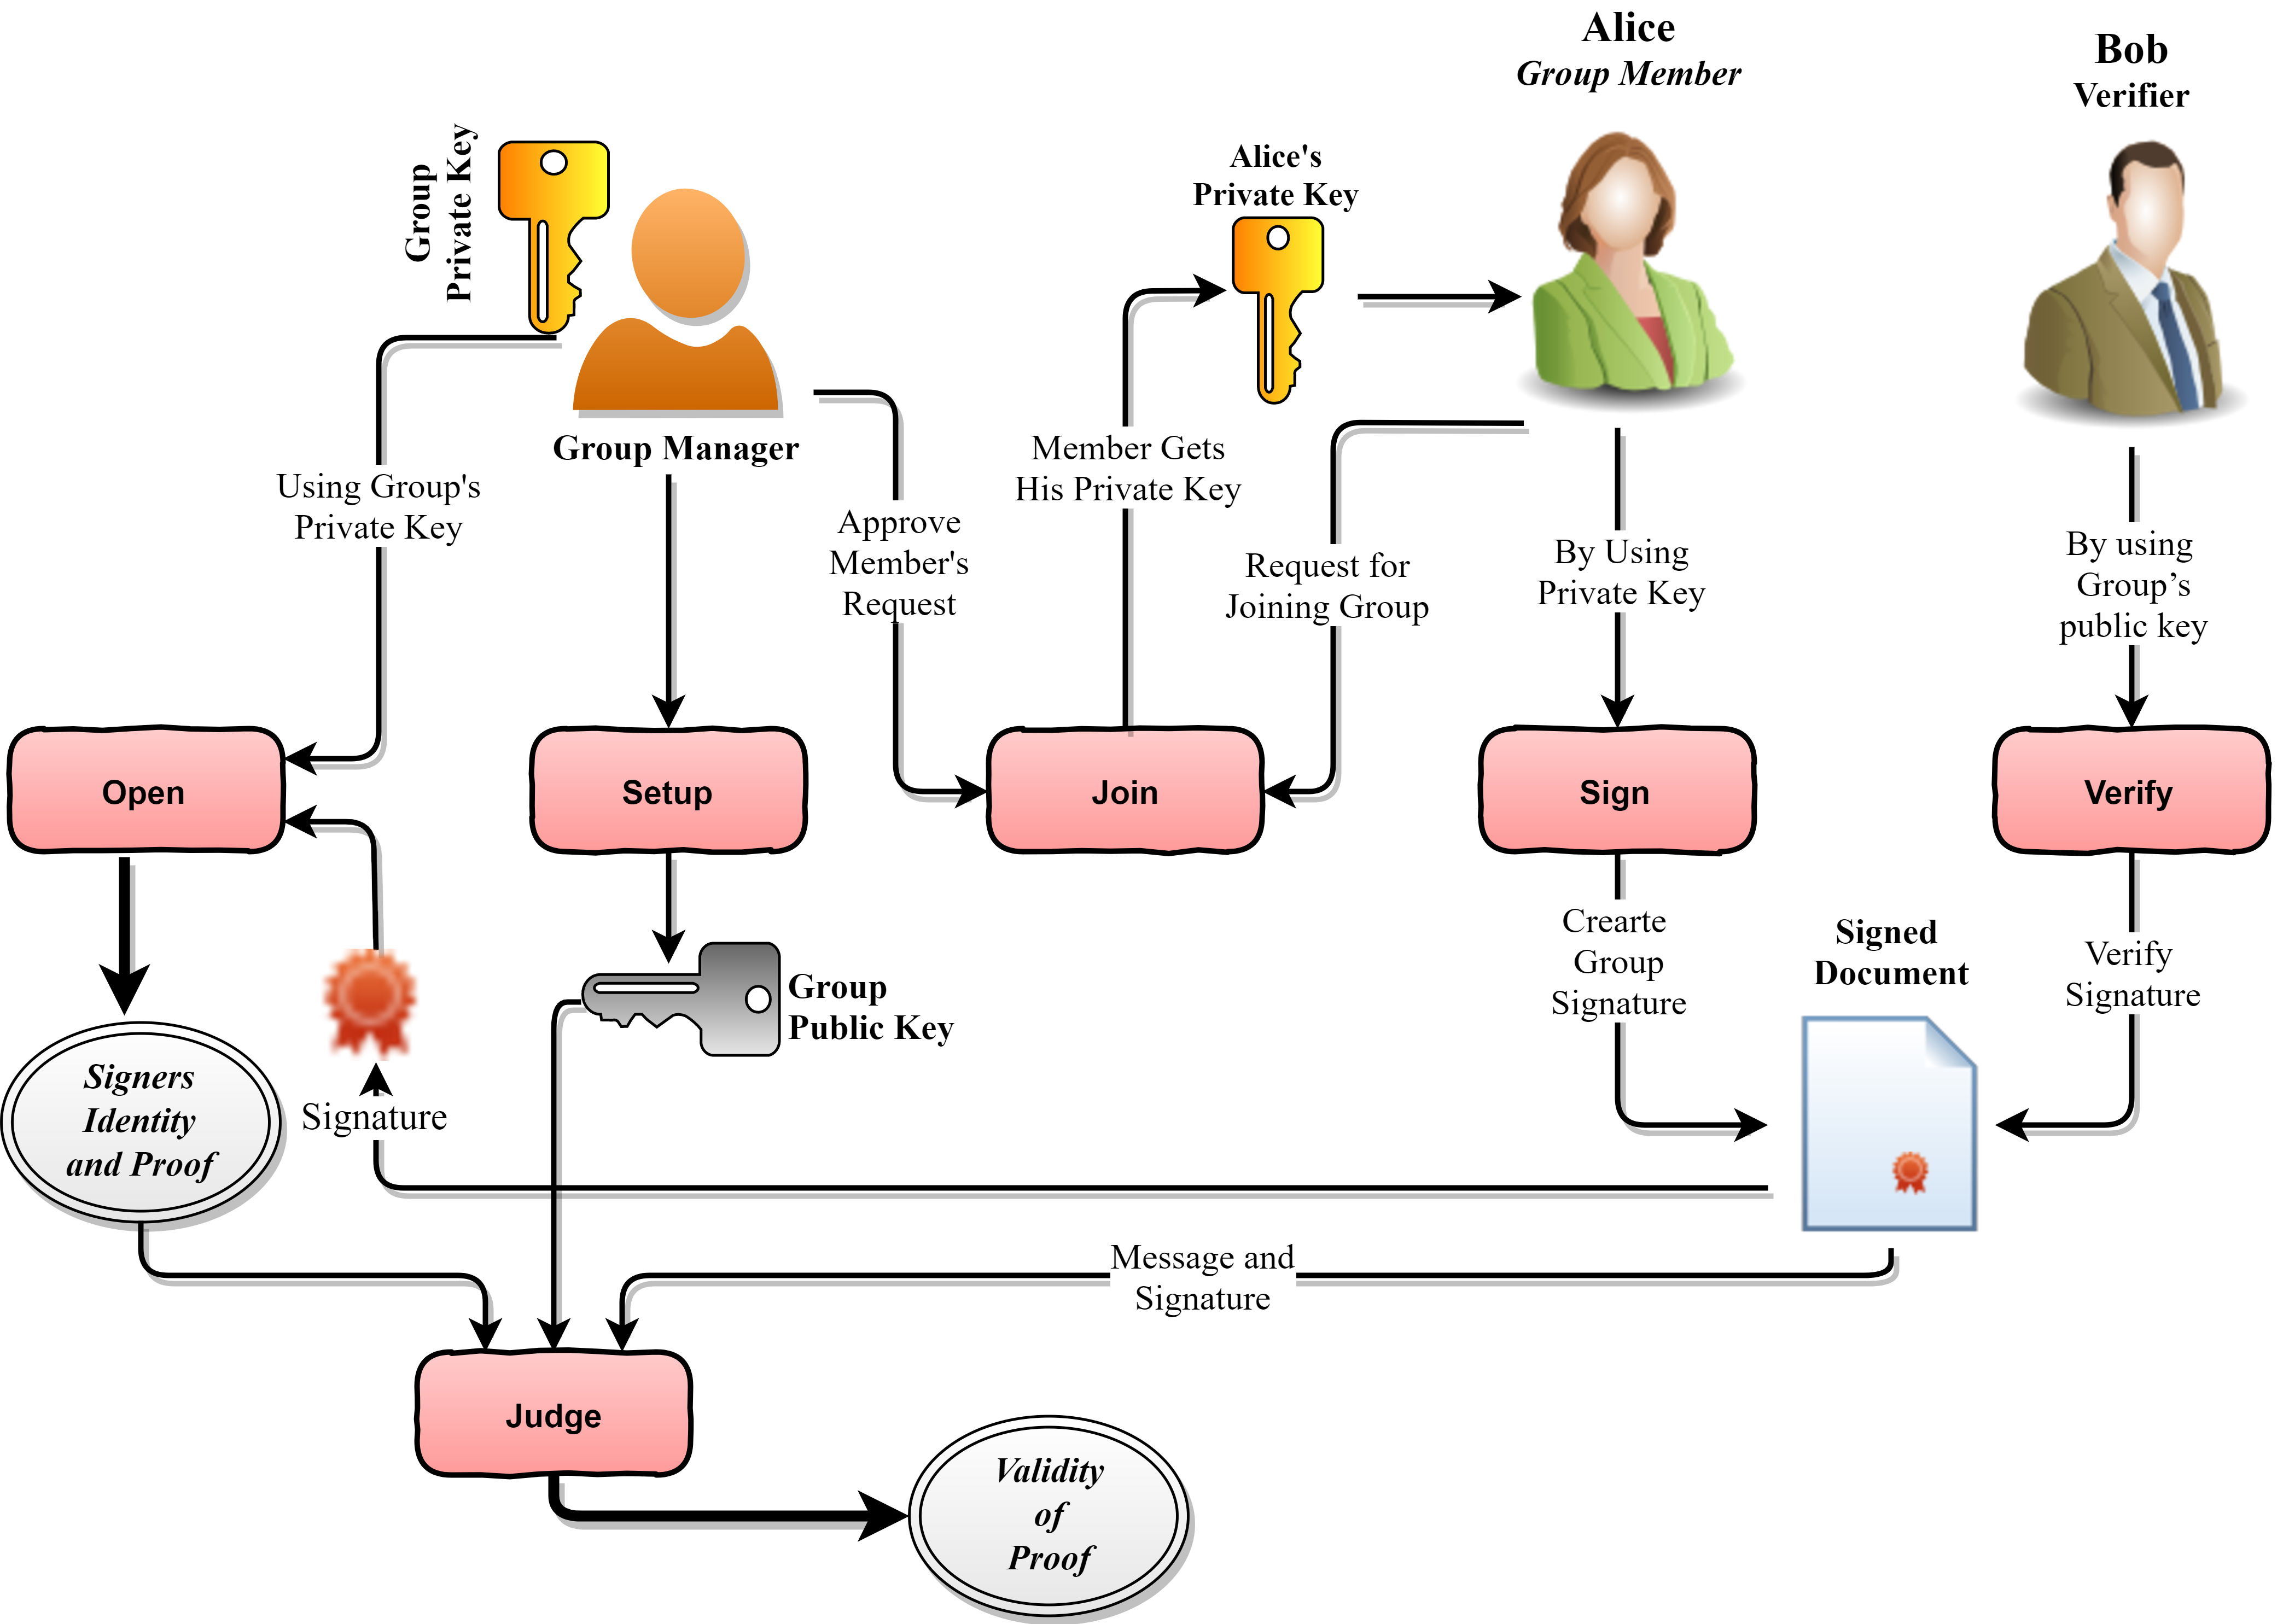
\includegraphics[width=\textwidth]{Publicverificableopeninggroupsignature}
    \caption{Group Signature Schemes with Verifiable Opening}
    \label{fig:Public verificable opening group signature}
\end{figure}
The figure \ref{fig:Public verificable opening group signature} shows the structure of publicly verifiable opening supported group signature scheme. In the figure, all the other components are similar to the dynamic group signature scheme and can be replaced with the static group signature scheme. The notable difference to those schemes is that the opening algorithm produces a proof along with the signer's identity. The supplementary algorithm Judge takes the input of the output of opening algorithm along with signature and message plus group public key and provides validity of the proof as an output. 

Note that the extension of the verifiable opening can be applied to both Static and Dynamic schemes because the extension only requires modification of opening algorithm which is present in both the schemes.

\subsection{Group Signature Schemes with Distributed Authorities}\label{sec:Group Signature Schemes with Distributed Authorities}
\index{group signature schemes with distributed authorities}The role of a Group Manager in a group signature scheme is one of the important roles as a trusted authority. In various schemes of group signatures, the Group Manager is responsible for various duties. To perform these functions, the members required to put a lot of trust in the Group Manager. Although we saw in previous schemes, Group Manager needed to provide publicly verifiable proof for an opened signature. It does not reduce the level of trust required in Group Manager's role. One important solution to those problems is to distribute the tasks of Group Manager among multiple separate entities. It helps in migrating the amount of trust in Group Manager and suites for some specific applications where trust is not required, and separation is necessary for architecture of the group signature scheme. 

The important tasks that a Group Manager is supposed to be responsible are, the generation of the private and public key of the group, opening the signature, revocation of the members in the revocation supported schemes, distribution of private keys of the members in static and joining of the member in dynamic schemes. All these tasks required in common is the private key of the group. So if the mathematical foundation of the group signature can be constructed in such a way that separate private keys are required for performing the tasks mentioned above, it is possible to distribute the role of Group Manager into various authorities. The essential functions of the distributed authorities are as follows.

The first task is the generation of the private and public key of the group, as well as the distribution of private keys to the members in static and joining the members in dynamic schemes, can be assigned to a separate authority called as the \texttt{Issuer}. An another authority can be assigned the task of opening the signature. This authority possesses a unique opening key, which can associate a signature to its signer. This type of authority is known as the \texttt{Opener}. If the scheme supports revocation of the members, the task of the revocation can be assigned to a separate authority called the \texttt{Revocator}. Some architecture may also suggest that when opening authority identifies the signer of a signature, it can also send a request to the revocation authority to revoke that member along with the identity of the signer and only then revocation authority can revoke such member.
\begin{definition}[Group Signature Scheme with Distributed Authorities]\label{def:Group Signature Scheme with Distributed Authorities}The group signature scheme with distributed authorities, is a static or dynamic group signature scheme in which \texttt{SetUp}, \texttt{Open} and \texttt{Join} algorithms are modified in such a way that different private keys are required for their execution.\\
\textbf{SetUp:} The randomized \texttt{SetUp} algorithm produces a tuple $(gpk, gsk\lbrack~\rbrack, list)$ by taking an input of security parameter $(1^k, k \in \mathbb{N})$ where $gsk$ is the private key of the authority is an array denoting $gsk\lbrack i \rbrack$ is a private key of the authority $i$.\\
\textbf{Join:} The randomized \texttt{Join} algorithm is a protocol between the issuer and a user which takes input $gsk\lbrack Issuer \rbrack$ and provide $mpk$ to the user which is his private key.\\
\textbf{Open:} The deterministic algorithm \texttt{Open} returns $mpk$ of signer member by taking input $(gsk\lbrack Opener \rbrack, S)$ where $S$ is the signature of a message.
\end{definition}
\begin{figure}[h]
    \centering
    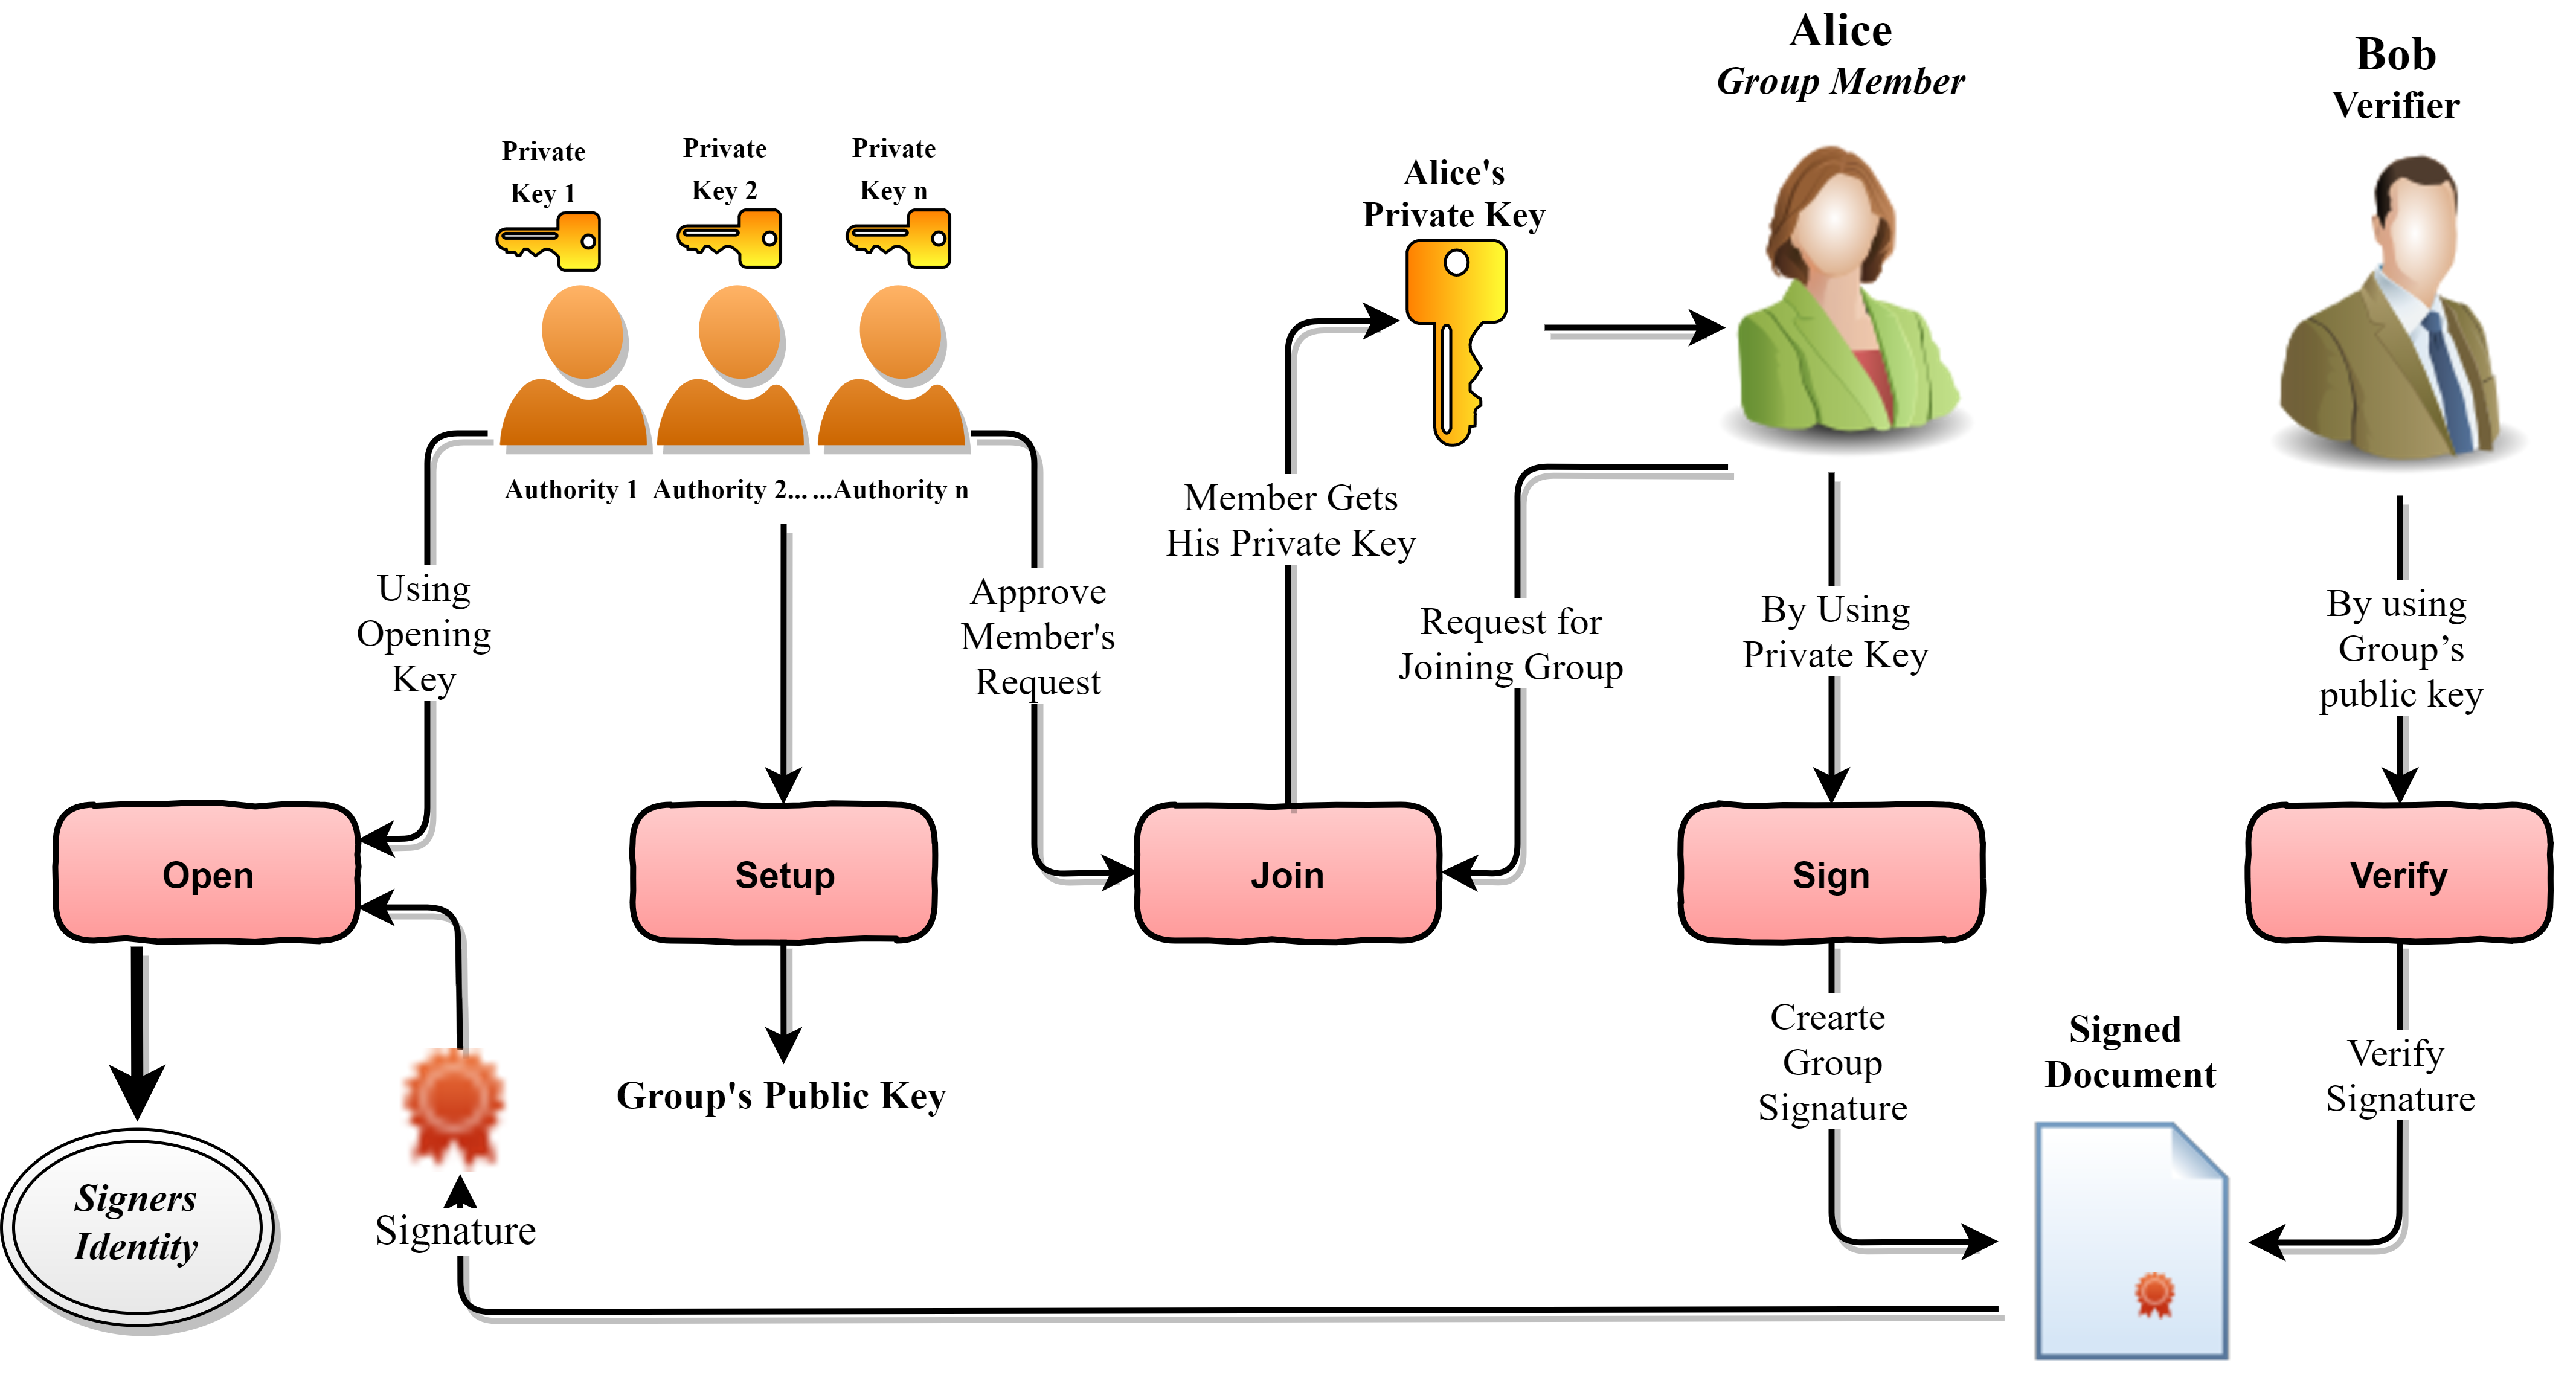
\includegraphics[width=\textwidth]{groupsignaturewithdistributedauthorities}
    \caption{Group Signature Schemes with Distributed Authorities}
    \label{fig:Group Signature Schemes with Distributed Authorities}
\end{figure}
The figure shows architecture of group signature scheme with distributed authorities. In the figure, various authorities are shown that are responsible for different tasks. One authority is responsible for generating the public key of the group, another authority is responsible for joining the members in the group, and the role of the opening signature is assigned to separate authority. Each authority in the figure is in possession of the different private key. The role of signer and verifier are similar to that of other group signatures schemes.

\subsection{Group Signatures with Unique Properties}\label{subsection:GSUniqueProperties}
Although the classification of the group signatures in the earlier section covers most of the group signatures schemes, some schemes are not included in it. Those schemes have a unique construction whose properties are not comparable with most of the common group signature schemes.
\subsubsection{Blind Group Signature}
A Blind group signature\index{blind group signature} scheme is a combination of blind signatures and group signatures. The blind group signature work in the following manner. A group signature is generated in such a way that signer should not be able to see the message $M$, which chosen by a third party. The third party also does not know the identification of the signer. After concluding this interaction, the third party gets a valid group signature for the message $M$, and signer doesn't have any knowledge of the message or the signature produced by his private key.

Lysyanskaya proposes the application of this fascinating structure\cite{lysyanskaya1998group}. The purpose of the application of blind group signatures is that the signature generation process should be unlinkable to the message as well as the signature. Application of Lysyanskaya describes an electronic cash system in which issuer bank is the blind signer, and the signed message can be considered as an electronic currency. As a part of a financial group, the issuer bank provides the electronic money to a customer at the time of withdrawal, and the customer can use this currency for transactions without revealing any information about the issuer bank as well as disabling the issuer bank to track the utilization of this electronic currency by the client.

\subsubsection{Democratic Group Signature}
The mathematical structure of Democratic group signature\index{democratic group signature} is built in such a way that the need for authorities, especially the Group Manager is eliminated\cite{manulis2006democratic}\cite{manulis2006linkable}. Instead, the tasks of Group Manager are executed by the group members. The group members can work democratically because the scheme provides such a unique power to all the group members. The addition and revocation of the members are done jointly, where members are required to agree in a majority. The opening of the signature is done by each member individually. Here each member has the ability to link any signature to its original signer. The verifier, who are not group members are still unable to link the signature to its original signer, and signatures remain anonymous to the verifiers. 

Some democratic group signature scheme can restrict the opening ability to a limited subset of group members\cite{li2009}. Some schemes allow the signer to decide such subset of members having the opening ability\cite{li2009democratic}. In those schemes, each subset of members can open specific signatures but not all the signatures.

\subsubsection{Mediated Group Signature}
In the Mediated group signature\index{mediated group signature} scheme an additional entity named the Mediated Server is present\cite{ding2004leak}. This entity is required for generation of the signatures by group members. For generating a signature a signer required to identify themselves to the Mediator server and provide a partial signature. After getting the partial signature, the mediating entity is able to generate full group signature if the signer is not revoked. The mediation entity is also useful in the revocation of the members. The mediated entity maintains a list of revoked members and adds a member in the list on the request of the Group Manager. The mediated group signature has a unique security property known as leak-freedom. The leak-freedom property prevents the group members from producing past signed signatures.

\section[Group Signature Schemes based on General Assumptions]{Group Signature Schemes based on \\General Assumptions}
To implement the group signature scheme some authors proposed a different way which was based on generic solutions and uses cryptographic primitives in a black box way. Which means in simple terms the scheme is constructed using the schemes and algorithms which were already devised and used for different purposes. Although these type of systems are found to be less efficient than the schemes based on number theoretical assumptions, they provide the need of hardness assumption to prove security and also elaborate some design specifications required for security of the group signature schemes. Following section represent some notable group signature schemes which are based on general assumptions. These schemes use the \textquotedblleft sign and encrypt and prove\textquotedblright ~ pattern which is also employed in some other group signatures.

\subsection{The Bellare Micciancio Warinschi Scheme}
The construction of The Bellare Micciancio Warinschi Scheme\index{Bellare Micciancio Warinschi Scheme} (hereinafter referred as the BMW scheme) is based on digital signature scheme, asymmetric key encryption and noninteractive zero-knowledge protocol for proof of knowledge\cite{bellare2003foundations}. The BMW scheme builds on the generic scheme proposed by Camenisch and Michels\cite{camenisch1999separability}. 

The generic algorithms in cryptography used by the BMW scheme are:
\begin{itemize}
\item A digital signature scheme $DS$ = (Key Generation, Sign, Verify).
\item An asymmetric encryption scheme $PKE$ = (Key Generation, Encrypt, Decrypt).
\item A noninteractive zero-knowledge protocol for zero knowledge proof.
\end{itemize}

In the BMW scheme, the private key of a member $i$ is made up of a secret key $sk_i$ and a Digital Certificate $Cert_i$, which was issued by the Group Manager. Therefore the certificate can be viewed as the certificate of Group Manager on member's public key. To generate a signature for a message $M$, the member $i$  encrypts $(i, pk_i, Cert_i)$ by using the public key of the group $gpk$. Then the member generates digital signature $S$ by using $sk_i$ on message $M$ and provide a proof of knowledge by the noninteractive zero-knowledge protocol. For verification of the signature $S$, a verifier provides an input of $gpk$, message $M$ and signature $S$ to the \texttt{Verify} algorithm, which parses the signature $S$ and validate the zero knowledge proof given by the signer in the signature. To associate a signature to its signer, the Group Manager decrypts the $(i, pk_i, Cert_i)$ by using $gsk$ and find out the identity of the signer using $cert_i$. 

The BMW scheme does not support verifiable opening and accusation a member by Group Manager is possible. The zero-knowledge proof provided by the group member can be extended in such a way that accusation of members should not be possible. The BMW scheme is a static group signature scheme and does not support the addition of any new members after the commencement of the group, but the revocation of any member can be done by making some modifications in the scheme. By default, the proposed scheme does not have any member revocation mechanism in it. The BMW scheme provides various security properties like nonframeability and traceability. The scheme also satisfies full anonymity defined in \cite{bellare2003foundations} called as Beller's model of Group Signature. The modified adaptation of this system which supports the addition of members after the creation of the group and enhanced security is explained in the next section.

\subsection{The Bellare Shi Zhang Scheme}
The Bellare Shi Zhang scheme\index{Bellare Shi Zhang scheme} is a dynamic group signature scheme created using generic algorithms\cite{bellare2005foundations}. The scheme not only provides a verifiable opening but also distributes the task of Group Manager into two separate authorities. One authority is responsible for issuing the $mpk$ and joining the members who called the \texttt{Issuer} and another authority responsible for associating the signature to its original signer named as the \texttt{Opener}. The scheme also implements a system of user PKI for possible members. The Bellare Shi Zhang scheme is very much similar to the static BMW scheme and uses a unforgeable digital signature scheme, an asymmetric encryption algorithm and two noninteractive zero-knowledge protocol for zero knowledge proofs. 

The \texttt{SetUp} algorithm of the Bellare Shi Zhang scheme uses both the digital signature scheme and asymmetric encryption scheme to generate private keys of the \texttt{Issuer} and the \texttt{Opener} in the following fashion. First, two common reference strings are calculated by taking an input of parameter $1^k, k \in \mathbb{N}$. Then a public and private key pair is generated for the digital signature scheme, and another public and private key pair is generated for the asymmetric encryption algorithm. The public key of the group is a tuple of the two common reference strings and both public keys of digital signature and asymmetric encryption algorithm. The private key of the \texttt{Issuer} is the private key of the digital signature scheme, and the private key of the \texttt{Opener} is the private key of the asymmetric encryption algorithm. The \texttt{SetUp} algorithm also generates a $List$ of users which is empty at the beginning. 

The \texttt{Join} protocol of the scheme is required to be executed in a secure channel because of the transmission of the private key and $cert_i$ of the member. In this system, the user generates his own private and public key pair for the digital signature scheme and get $cert_i$ from the \texttt{Issuer}, and the public key of the user is stored in the $List$.

The signature generation and signature verification procedure are exactly same as the BMW scheme which is discussed in the previous section. Whereas, the \texttt{Open} algorithm is also similar to the BMW system, except the addition of the signer's identity and the requirement of a separate private key of the \texttt{Opener} for opening the signature. The \texttt{Open} algorithm of this scheme also provides a publicly verifiable proof of the opened signatures which can be verified by using the \texttt{Judge} algorithm. Revocation mechanism is not provided in the proposed scheme, but an extension is possible
%by various mechanisms like verifier-local revocation 
to allow revocation.
% of a member. 

The security of the Bellare Shi Zhang scheme is similar to that of the BMW scheme and provides full anonymity, traceability, and nonframeability. The nonframeability is the additional security property present in this scheme than the BMW scheme.

\section[Group Signature Schemes using RSA assumption]{Group Signature Schemes using\\ RSA assumption}
\index{group signature schemes using RSA assumption}The RSA\nomenclature{RSA}{Rivest, Shamir, and Adleman algorithm for asymetric cryptography} assumption is found to be useful not only for the digital signatures schemes but also for the group signature schemes. An earlier scheme, which uses the RSA assumption, was proposed by D. Chaum\cite{chaum1991group}. This proposed scheme had some shortcomings in it like the security requirements were not entirely satisfied as of modern needs. Also in that scheme, the length of the group public key and the signature was quite long. The scheme was a static signature scheme and does not support the later addition of members in the group. A dynamic scheme, which is based on the RSA assumption was proposed by Camenisch and Stadler\cite{camenisch1997efficient}. Their scheme produces a uniform length of signature and group keys. The scheme of Antenies and Tsudik offers a more efficient variant with dynamic group signatures\cite{ateniese1999group}. Whereas, the scheme proposed by Camenisch and Michels was also efficient static group signature with a verifiable opening algorithm\cite{camenisch1998group}. All these schemes use the RSA assumption as a base for their security. 

None of the schemes mentioned above offers revocation of a member from the group, but several extensions were offered to deal with this shortcoming. The article of Bresson and Stern proposes a modification of the Camenisch and Stadler scheme\cite{camenisch1997efficient} to enable revocation of group members\cite{bresson2001efficient}. The extension of Ateniese et. al. \cite{ateniese2002quasi} uses noninteractive zero-knowledge proofs for revocation procedure in the ACJT scheme. Camenisch and Lysyanskaya proposed an out of the box solution of using dynamic accumulators for the purpose of revocation of members in the group signature scheme\cite{camenisch2002dynamic}. 

The group signature scheme of Nakanishi and Sugiyama was a dynamic group signature scheme with distributed authorities\cite{nakanishi2004group}. An amendment of this scheme was also proposed by Nakanishi for efficient update of members private key for unrevoked group members but increases the load of Group Manager\cite{nakanishi2005group}. The paper of Camenisch and Groth proposes multiple group signature schemes based on RSA assumption\cite{camenisch2004group}. These schemes were static and dynamic in nature and support revocation of members. The next section provides a detailed discussion about some important group signature schemes which are based on the RSA assumption.

\subsection{The ACJT Scheme}\label{ACJT}
This section elaborates the group signature scheme introduced by Ateniese, Camenisch, Joye, and Tsudik\cite{ateniese2000practical}. This scheme is a dynamic group signature scheme and popularly known as the ACJT scheme\index{ACJT scheme}. This scheme has been adapted from numerous schemes like the Camenisch and Stadler scheme\cite{camenisch1997efficient}, Camenisch and Michel scheme\cite{camenisch1998group} and Ateniese and Tsudik scheme\cite{ateniese1999group} which were discussed in the previous section. 

The unique advantage of the ACJT scheme is that the practical implementation of the scheme was possible. The scheme provides a verifiable opening procedure and has the ability to generate group public and private keys along with the signature with uniform length. The scheme was also resistant to the coalition of members attack, which is an essential security requirement for a group signature scheme. The security of the scheme was not only dependent on the RSA assumption but also the quadratic reciprocity assumption and Diffie-Hellman assumption were used to enhance the security. The scheme was able to implement almost all the modern security properties required for a group signature scheme and mathematical proofs of that are also provided for them. 

The scheme defines a set of security parameters $\lambda_2, \lambda_1, \gamma_2, \gamma_1$ and ranges $\Gamma, \Lambda$ in the following way.
\[
\lambda_2 \geq 4\ell_p, 
\lambda_1 \geq \varepsilon(\lambda_2 + k) + 2 , 
\gamma_2 \geq \lambda_1 + 2 , 
\gamma_1 \geq \varepsilon(\gamma_2 + k)+ 2 ,
\]
\begin{center}
and ranges $\Gamma = ]2^{\gamma_1-\gamma_2}, 2^{\gamma_1+\gamma_2}[$ and 
		   $\Lambda = ]2^{\lambda_1-\lambda_2}, 2^{\lambda_1+\lambda_2}[$.
\end{center}

\subsubsection{SetUp}
The \texttt{SetUp} algorithm of the ACJT scheme uses two large prime numbers $p^\prime$ and $q^\prime$ in the strong RSA assumption and calculate the RSA modulus as $n = (2p^\prime + 1)(2q^\prime + 1)$. The public and private keys of the group are generated in the following manner.

\begin{algorithm}
\caption{\texttt{SETUP} of ACJT scheme}
\begin{algorithmic}[1]
\STATE Generate random numbers $g, h, a, a_0 \in \operatorname{QR}(n)$ and of order $p^\prime q^\prime$.
\STATE Select random $x$ and calculate $y = g^x (mod~n)$
\STATE Group Manager sets group's public key as \framebox[1.1\width]{$\mathcal{Y} = (n, a, a_0, y, g, h)$}.
\STATE Group Manager sets group's private key as \framebox[1.1\width]{$\mathcal{S} = (p^\prime, q^\prime, x)$}.
\end{algorithmic}
\end{algorithm}

In the \texttt{SetUp} phase, the RSA modulus is assumed to be safe and in possession of a trusted party. The public key elements $(g, h, a, a0)$ selected randomly from $QR(n)$.

\subsubsection{Join}
The \texttt{Join} algorithm is a protocol between Group Manager and a user, resulting the user becoming a member of the group by getting his private key. The \texttt{Join} algorithm of the ACJT scheme is more secure than previous schemes and uses zero-knowledge proof. The procedure of the \texttt{Join} algorithm is as follows.

\begin{algorithm}
\caption{\texttt{JOIN} protocol of ACJT scheme}
\begin{algorithmic}[1]
\STATE User $U_i$ generate random exponent $\hat{x}_i \in_R ]2, 2^{\lambda_2}[$ and random number $\hat{r} \in_R ]0, n^2[$ then send $C_1 = g^{\hat{x}_i}h^{\hat{r}}(mod~n)$ to Group Manager. also proves his knowledge of $C_1$.
\STATE Group Manager verifies $C_1 \in \operatorname{QR}(n)$, if verified, then selects $\alpha_i$ and $\beta_i$ $\in_R ]2, 2^{\lambda_2}[$ and sends $\alpha_i$ and $\beta_i$ to user $U_i$.
\STATE User $U_i$ computes $x_i = ( \alpha_i \hat{x}_i + \beta_i (mod~2^{\lambda_2})) + 2^{\lambda_1} $ and sends $C_2 = a^{x_i}(mod~n)$. User $U_i$ also provide zero-knowledge proof for $C_2$.
\STATE Group Manager checks $C_2 \in \operatorname{QR}(n)$. If it is, then selects a random prime $E_i \in_R \Gamma$ and calculate
\framebox[1.1\width]{$A_i = (C_2 a_0)^{E_i^{-1}} (mod~n)$}
and send $U_i$ membership certificate $[A_i, E_i]$
\STATE User $U_i$ verifies if $a_0 a^{x_i} = A_i^{E_i} (mod~n)$.
\end{algorithmic}
\end{algorithm}

\subsubsection{Sign}
To generate a signature for a message, the user required his private key and group public key. The method of generating a signature is as follows.
\begin{algorithm}
\caption{\texttt{SIGN} algorithm of ACJT scheme}
\begin{algorithmic}[1]
\STATE Signer generate random number $w \in_R \{ 0,1 \}^{2\ell_P}$ and calculate 
$T_1 = A_i y^w (mod~n)$,
$T_2 = g^w (mod~n)$,
$T_3 = g^{e_i}h^w(mod~n)$.
\STATE Generate random number
$r_1 \in_R \pm \{ 0,1 \}^{\varepsilon(\gamma_2 + k)}$, 
$r_2 \in_R \pm \{ 0,1 \}^{\varepsilon(\lambda_2 + k)}$, 
$r_3 \in_R \pm \{ 0,1 \}^{\varepsilon(\lambda_1 + 2\ell_p + k + 1)}$,
$r_4 \in_R \pm \{ 0,1 \}^{\varepsilon(2\ell_p + k)}$.
and calculate
$d_1 = T_1^{r_1} / a^{r_2}y^{r_3} (mod~n)$,
$d_2 = T_2^{r_1} / g^{r_3} (mod~n)$,
$d_3 = g^{r_4} (mod~n)$,
$d_4 = g^{r_1}h^{r_4}(mod~n)$.\\

\framebox[1.1\width]{$C = \mathcal{H}(g\parallel h\parallel y\parallel a_0 \parallel a\parallel T_1\parallel T_2\parallel T_3\parallel d_1\parallel d_2\parallel d_3\parallel d_4\parallel M)$}.\\

$s_1 = r_1 - C(E_i- 2^{\gamma_1})$,
$s_2 = r_2 - C(x_i- 2^{\lambda_1})$,
$s_3 = r_3 - C E_i w$,
$s_4 = r_4 - C w$. in $\mathbb{Z}_n^*.$

\STATE Output \framebox[1.1\width]{$(C, s_1, s_2, s_3, T_1, T_2, T_3)$}.
\end{algorithmic}
\end{algorithm}

Note that a separate ElGamal encryption\cite{elgamal1985public} is required to generate the $T1$ and $T2$.

\subsubsection{Verify}
To verify a signature, verifier required the public key of the group along with the signature and the message. The verifier verifies the signature in the following manner.
\begin{algorithm}
\caption{\texttt{VERIFY} algorithm of ACJT scheme}
\begin{algorithmic}[1]
\STATE Calculate $C^\prime = \mathcal{H}(g\parallel h\parallel y\parallel a_0\parallel a\parallel T_1\parallel T_2\parallel T_3\parallel
\frac{(a_0^C T_1^{s_1-C2^{\gamma_1}})} {(a^{s_2-C2^{\lambda_1}}y^{s_3})}
\parallel \frac{(T_2^{s_1- C2^{\gamma_1}})}{g^{s_3}}
\parallel T_2^C g^{s_4}
\parallel (T_3^C g^{s_1-C2^{\gamma_1}} h^{s_4}
\parallel M) $.
\STATE Signature is valid if and only if $C = C^\prime$ and 
$s_1 \in \{ 0, 1\}^{\varepsilon(k + \gamma_2)+1}$,
$s_2 \in \{ 0, 1\}^{\varepsilon(k + \lambda_2)+1}$,
$s_3 \in \{ 0, 1\}^{\varepsilon(k + \lambda_1+2\ell_p + 1)+1}$,
$s_4 \in \{ 0, 1\}^{\varepsilon(k + 2\ell_p) + 1}$.
\end{algorithmic}
\end{algorithm}

\subsubsection{Open}
To associate a signature to its original signer, the Group Manager performs the following procedure using his private key.
\begin{algorithm}
\caption{\texttt{OPEN} algorithm of ACJT scheme}
\begin{algorithmic}[1]
\STATE Verify the validity of signature by \texttt{VERIFY} algorithm.
\STATE Calculate $A_i$ (The identity of $U_i$) as \framebox[1.1\width]{$A_i = T_1/T_2^x$}.
\STATE Provide Proof that $\log_g y = \log_{T_2}{T_1 / A_i}$.
\end{algorithmic}
\end{algorithm}

The \texttt{Open} algorithm of this scheme also provides a noninteractive zero-knowledge proof to avoid framing of a member by the Group Manager.

\subsubsection{Security of the ACJT scheme}
The ACJT scheme is a Pioneer in providing a most secure scheme with mathematical proofs that why this scheme is considered to be \textquotedblleft state of the art\textquotedblright. The scheme provides full anonymity as defined in Bellare strict model\cite{bellare2003foundations}. The scheme also found to be providing unforgeability, unlinkability, exculpability along with traceability and resistance to coalition.

\subsection{The Tsudik and Xu Scheme}\label{TX}
A dynamic variant of the ACJT scheme allowing revocation of members was suggested by Tsudik and Xu\cite{tsudik2003accumulating}\index{Tsudik and Xu scheme}. In this scheme the dynamic accumulator is formed by $n = n_1 * n_2$,  where $n_1$ and $n_2$ are big prime numbers and kept secret similar to the RSA modulus. The Tsudik and Xu scheme enable their group members to generate their own $n_i$ at the time of joining procedure, and the $n_i$ is placed in the accumulator by the Group Manager as a part of group public key. Group members use the knowledge of factorization of $n = n_1 * n_2$ to generate a signature for a message. The key generation mechanism of the Tsudik and Xu scheme is similar to ACJT scheme except the generation of dynamic accumulators at the commencement of the group. The public key and private key of the group are also very much similar to that of ACJT scheme. In the \texttt{Join} algorithm of this scheme, the user computes $n_i = n_1 * n_2$ and sends $n$ to the Group Manager. The Group Manager then adds the $n_i$ in accumulator after verifying it and sends user $acc_i$.

An important vulnerability of the scheme is that the accumulator is made up of composite numbers $n_i = n_{1i} * n_{2i}$, $n_j = n_{1j} * n_{2j}$ so a colluding attack it possible for members $i$ and $j$ because they can form some another values like $n_{1i} * n_{1j}$ , $n_{2i} * n_{2j}$ and forge a membership certificate that results into inadequate traceability. The \texttt{Sign} algorithm of this scheme is pretty much similar to the ACJT scheme except the use of accumulator in the signature generation and requirement of $T4$ and $T5$ values in the signature which apparently increases the size and cost of generation of the signature. The \texttt{Verify} algorithm and \texttt{Open} algorithm are also similar to ACJT scheme with slight modifications. The important contribution of the Tsudik and Xu scheme is the revocation mechanism which is done by updating the accumulator $acc_i$ in group public key as the $acc^{n_{i}^{-1} (mod~4 p\prime q\prime)} mod~N$ and replacing the entry of $n_i$ with \texttt{del}.

Apart from the security flaw mentioned earlier, the Tsudik and Xu scheme offers various security properties like nonframeability, unlinkability, and exculpability. The anonymity provided by this scheme is not full anonymity according to the  Bellare's model but partial anonymity (or simply anonymity). Similarly, full traceability is not offered by the scheme instead, only insider traceability is provided.

\subsection{The Camenisch and Groth Scheme}\label{CG}
The Camenisch and Groth scheme\index{Camenisch and Groth scheme} is a static group signature scheme which utilizes the RSA assumption\cite{camenisch2004group}. The Camenisch and Groth scheme is slightly faster than the ACJT scheme because of the modified Join algorithm. The basic scheme required a predefined number of group members to produce their private keys, and the Group Manager is an authority trusted to create and distribute private keys of the members. All the algorithms in this scheme similar to the Camenisch and Lysyanskaya scheme\cite{camenisch2002dynamic}. The original Camenisch and Groth scheme provides full anonymity and full traceability as well as nonframeability. The static nature of the scheme results in the limitation of some functionalities like the addition of new members is not possible also revocation of members is not described in the scheme. 

But to overcome these shortcomings, several modifications were recommended. The extension proposed by The Camenisch and Groth enables the later addition of members into the group, converting it to a dynamic group signature scheme. An algorithm for revocation of the members was also introduced which was similar to Camenisch and Lysyanskaya scheme's revocation algorithm where dynamic accumulators are used for the purpose of the revocation\cite{camenisch2002dynamic}. 

A separate extension was also introduced which incapacitates members from generating a valid signature from an old public key. This problem was addressed by combining the accumulator based approach with the local verification revocation approach. Those extensions provided not only same security properties as of the static version of the scheme but also offers full revocability and a verifiable opening of signatures.

\subsection{The Kiayias and Yung Scheme}\label{KY}
In this section, we are going to describe the scheme proposed by Kiayias and Yung\index{Kiayias and Yung Scheme}\cite{kiayias2005efficient}\cite{kiayias2006secure}. This scheme is not only a simple dynamic group signature scheme but also provides a verifiable opening procedure in it. The Kiayias and Yung scheme can be seen as the modification of ACJT scheme where RSA assumption is the base of the security. The setup algorithm of this scheme is almost same as the ACJT scheme except for the requirement of additional $\hat{y}$ and $\hat{x}$ in group public key and private key.

The \texttt{Join} algorithm of the scheme required the support of a third party to add a new member to the group. Also, it separates the member certificates from members private keys. In the \texttt{Sign} algorithm, new element $T_5$ was introduced and required two pairs of ElGamal encryption whereas in ACJT scheme only one pair was needed. The \texttt{Verify} and \texttt{Open} algorithms are similar to the ACJT scheme. 

The Kiayias and Yung scheme offers various security properties like full anonymity, full traceability, and nonframeability. But the extended length of the signature and number of elements in the key results in increased burden of computation to all members including Group Manager. The revocation of the members was not discussing this scheme, so no approach is available to enable the revocation of the members. To enable the distributed authorities the scheme divides the private key elements into two different authorities viz. \texttt{Issuer} and \texttt{Opener}.

\section[Group Signature Scheme using Discrete Logarithms]{Group Signature Scheme using \\ Discrete Logarithms}
\index{group signature using discrete logarithms}Although some group signature schemes use the discrete logarithm setting for their security, it appears that the discrete logarithm technique is not a very attractive setting for group signature schemes. In the discrete logarithms, group signature schemes are less efficient than the RSA schemes. Also, pure discrete logarithms are unable to implement the permutation trapdoor which is essential for the modern security of group signatures. Hence, most of the schemes in this domain uses a mixed setting where the use of RSA assumption is employed for additional security. 

The first scheme which uses discrete logarithm was proposed by Chen and Pedersen\cite{chen1994new}. Although, their scheme was dynamic in nature but can be considered as efficient. The length of generated signature was not fixed, and the security properties of this scheme were not sufficient like the scheme was vulnerable to coalition attack. Also associating a signature to its original signer required all the group members to cooperate with Group Manager. The scheme of Petersen also shows similar drawback as mentioned earlier\cite{petersen1998convert}. The following section provides a discussion of some notable group signature schemes which use the discrete logarithm setting for their security.

\subsection{The Ateniese de Medeiros Scheme}\label{AM}
A notable group signature scheme which uses dynamic logarithm setting was proposed by Ateniese and Medeiros\cite{ateniese2003efficient}\index{Ateniese de Medeiros Scheme}. The scheme allows verifiable opening of the signatures and dynamic addition of the group members. This scheme required a PKI system to distribute certificates to group members. The \texttt{SetUp} algorithm of this scheme required three security parameters and a trusted third party is assumed to be storing the strong RSA modulus. In the \texttt{SetUp} procedure of this scheme the parameters are calculated by determining a strong RSA modulus $\bar{P}$ where $\bar{P}= 2P + 1$ and $P= 2Q + 1$  and all $\bar{P}, P, Q$ are prime numbers. This secure RSA modulus is kept secure, and the parameters can be shared by multiple groups as long as the factorization of the modulus is not revealed. The \texttt{Join} algorithm of the scheme is a type of Nybra Rueppel Signature\cite{nyberg1996message} modified for using the public key of the group. 

The \texttt{Join} algorithm is required to be executed in a secure manner of communication so no intruder can identify the private key of the members. The signature is generated by this private key of the member, and two separate ElGamal encryptions are required for the signature elements similar to ACJT signature. The length of the signature depends on the length of the hash function used for the message. The verification of the signature is done by validating the proof of knowledge provided by the signer. 

The opening procedure is also a remarkably similar to the ACJT scheme where identification of the signer is generated by using $T_1$ and $T_2$ along with the private key of the group. The \texttt{Open} algorithm also produces a proof of knowledge for public verification. The scheme does not provide any security proof in \cite{ateniese2003efficient} except for the claim that the scheme is secure under random oracle model. This scheme provides anonymity but not full anonymity and traceability, and the proof of opening signature prevents framing attacks.

\subsection{The Furukawa Yonezawa Scheme}\label{FY}
The Scheme proposed by Furukawa and Yonezawa\index{Furukawa Yonezawa Scheme} is dynamic group signature scheme with distributed authorities\cite{furukawa2004group}. The scheme uses discrete logarithm assumption for its implementation and security. This scheme also provides a verifiable opening which provides a proof of correctly opened signatures by the Group Manager. This scheme also required a PKI system for key management. 

The key generation required a single parameter and strong RSA modulus which is assumed to be safe by a trusted third party. The \texttt{Join} protocol of this scheme is similar to the Ateniese de Medeiros Scheme and uses an adaptation of Nybra Rueppel Signature under Group Manager or in this case the \texttt{Issuer} of the public key. The \texttt{Sign}, \texttt{Verify} and \texttt{Open} algorithms are not very much different from the Ateniese de Medeiros Scheme and the ACJT scheme. 

Furukawa and Yonezawa provide various proofs and security of their scheme. The security properties of the scheme are traceability, full anonymity, and nonframeability. The scheme also provides an interesting extension in which multiple \texttt{Issuers} and multiple \texttt{Openers} can be implemented by using the threshold secret sharing techniques described by Pedersen in \cite{pedersen1991threshold}. 

\section{Other Notable Group Signature Schemes}
The RSA and discrete logarithms assumptions are not the only techniques used for implementing group signature schemes. Some remarkable group signature scheme uses different techniques than the technique discussed earlier. Those techniques involve bilinear maps pairing, elliptic curve cryptography, etc. The bilinear pairing maps are considered to be more efficient than the RSA or discrete logarithms to implement group signature schemes. Also, the elliptic curve cryptography which is found to be a more secure approach for public key cryptosystem is also found useful in implementing the group signature scheme. The following section describes some important schemes which use these techniques for their implementation.

\subsection{The Boneh Boyen Shacham Scheme}\label{BBS}
The group signature scheme proposed by Boneh, Boyen and Shacham is a static group signature scheme\index{Boneh Boyen Shacham Scheme} with distributed authorities\cite{boneh2004short}. The distributed authorities are accountable for the task of issuing the private key to the members and associating a signature to its original signer. This scheme is one of the first group signature scheme with uses bilinear pairing in its implementation. The \texttt{SetUp} algorithm of this scheme requires single security parameter and bilinear groups $\mathbb{G}_1 = \langle g_1\rangle$, $\mathbb{G}_2 = \langle g_2\rangle$ and $\mathbb{G}_p$ of prime order $Q$ and a bilinear map $\OE = \mathbb{G}_1 \mathbb{G}_2 \rightarrow \mathbb{G}_p$ and homomorphism $\Psi$ from $\mathbb{G}_2$ to $\mathbb{G}_1$ where $\Psi(g_2) = g_1$.

As the scheme is a static group signature scheme, the \texttt{SetUp} algorithm required  $n$, as a number of group members along with parameter $1^k$ and produces group public key and private key as well as $n$ private keys of the members and registration number for each member. Note that the private key is divided into two separate parts that are \texttt{Issuer's} private key and \texttt{Opener's} private key. The key distribution is required to be performed in a trusted manner as it carries the private key of the members. 

The signer uses his private key and group public key to generate a signature and produce $T_1, T_2, T_3$ as a linear encryption of private key and a signature of knowledge which proves that the signer possesses the private key that can be opened by the opening authority. The verifier uses the proof of knowledge for verification of the signature. The opening entity can associate a signature to its signer but does not provide any proof of knowledge. The scheme provides full anonymity and insider traceability but only provides insider nonframeability and not full nonframeability. 

The paper of Boneh, Boyen, and Shacham also provides an extension which enables revocation of members from the group. This revocation process perhaps reduces the security of the scheme. Another extension of this scheme converts the static scheme into a dynamic scheme and introduces additional \texttt{Join} algorithm for the addition of the members into the group. This extension indeed preserves all the security properties of the original scheme, but revocation of the members is not supported in this extension.

\subsection{The Camenisch Lysyanskaya Scheme}\label{CL}
The scheme proposed by Camenisch and Lysyanskaya\index{Camenisch Lysyanskaya Scheme} was one of the primary group signature scheme constructed by using bilinear maps\cite{camenisch2004signature}. The scheme is dynamic group signature scheme with distributed authorities. The distributed authorities are the \texttt{Issuer} and the \texttt{Opener}. The \texttt{SetUp} of the group is required to be performed in a trusted manner and all the elements required should be chosen at random to guarantee the confidence in the group public key. 

The scheme uses the Cramer Shoup encryption system to generate the private key of the group\cite{cramer1998practical}. The Cramer Shoup cryptosystem is secure under decisional Diffie Hellman assumption. By using the \texttt{Join} algorithm, new members are added to the group. This \texttt{Join} algorithm is needed to be executed in a secure channel to protect the membership certificate from intruders. The Sign algorithm also a derivative of the Cramer Shoup cryptosystem. The proof of knowledge is produced to prove the signer’s knowledge of the private key. The verification is similar to Boneh, Boyen and Shacham scheme and the \texttt{Open} algorithm does not provide any knowledge of proof for Group Manager. Hence the procedure is susceptible to frameability. The scheme provides its security by using Beller’s model and provide full anonymity and insider traceability along with partial traceability. 

\subsection{The Bichsel Camenisch Neven Smart Warinschi Scheme}\label{BCNSW}
The scheme proposed by Bichsel et. al.\index{Bichsel Camenisch Neven Smart Warinschi Scheme} is a dynamic group signature scheme with a verifiable opening\cite{bichsel2010get}. The scheme also requires a user PKI system for members. The attractive feature of this scheme is that it does not follow a typical \textquotedblleft sign encrypt and prove\textquotedblright procedure like other group signature scheme. Also, it provides the shortest signature size and minimum computational time while providing strong security. The PKI of the system uses a unforgeable digital signature scheme. The \texttt{SetUp} of the scheme requires bilinear groups and bilinear maps and two hash functions as random oracles. 

In the key generation process, the PKI system is used to generate the private and public key pair for the group. The \texttt{Open} algorithm takes a linear time according to the number of members. Therefore the Group Manager requires ample resources to open a signature. The \texttt{Open} algorithm also provides a zero knowledge proof for public verification of opening and therefore framing of a member is not possible. The Bichsel et. al. scheme provides security properties like anonymity but not full anonymity and insider traceability and nonframeability. The table \ref{table:variousgroupsignatures} shows different group signatures discussed in this section.
\begin{table}[!h]
\begin{center}
\begin{threeparttable}
\renewcommand{\arraystretch}{1.3}
\caption{Various group signatures schemes.}
\label{table:variousgroupsignatures}
\small
\begin{tabular}{| >{\arraybackslash}m{2.2in} |>{\centering\arraybackslash}m{0.55in} |>{\centering\arraybackslash}m{0.9in} |>{\centering\arraybackslash}m{0.5in} |>{\centering\arraybackslash}m{0.7in} |}
\hline 
\textbf{Group Signature scheme by} & \textbf{Short} & \textbf{Assumption} & \textbf{Section} & \textbf{Refrence}\\ 
\hline\hline
Ateniese Camenisch %
et.al.	 			& ACJT	& RSA & \ref{ACJT}& \cite{ateniese2000practical}  \\ \hline
Tsudik and Xu 		& TX	& RSA & \ref{TX}  & \cite{tsudik2003accumulating} \\ \hline
Camenisch and Groth	& CG	& RSA & \ref{CG}  & \cite{camenisch2004group}\\ \hline
Kiayias and Yung	& KY	& RSA & \ref{KY}  & \cite{kiayias2005efficient}\\ \hline
Ateniese de Medeiros& AM	& DL  & \ref{AM}  & \cite{ateniese2003efficient}\\ \hline
Furukawa Yonezawa	& FY	& DL  & \ref{FY}  & \cite{furukawa2004group}\\ \hline
Boneh Boyen Shacham	& BBS	& BM  & \ref{BBS} & \cite{boneh2004short}\\ \hline
Camenisch Lysyanskaya& CL	& BM  & \ref{CL}  & \cite{camenisch2004signature}\\ \hline
Bichsel Camenisch %
et.al.				& BCNSW	& BM  &\ref{BCNSW}& \cite{bichsel2010get}\\ \hline
\end{tabular}
\end{threeparttable}
\end{center}
\end{table}

\section[Similar Approaches for Authentication with Privacy]{Similar Approaches for Authentication with \\Privacy}
There are some other methods that are proposed to maintain privacy while providing authentication. Although these methods were proposed for different objectives, a lot of them have similar functionality as of the group signatures. That's why these approaches are not group signature, but they are constructed using similar cryptographic foundations as of the group signatures. Also, some strategies of these approaches are similar to group signatures. Following section describe some interesting concepts which are not only analogous to the group signatures but also have similar functionality.

\subsection{Affiliation Hiding Authentication}
The affiliation hiding\index{Affiliation Hiding Authentication} is a protocol composed for implementing authentication while preserving privacy. The concept of affiliation hiding is similar to group signature where it protects members identity by using group based authentication. But the affiliation hiding authentication also masks the identity of the group whereas in group signature authentication the identity of the group is not disguised. The affiliation hiding protocol generally classified into two varieties one is secret handshake protocol, and other is key establishment protocol. The authentication is done by matching the affiliation of both parties in which a viable communication is required. If the affiliation is matched, then the parties become authenticated else protocol gets terminated without providing any knowledge other than the not matching of the affiliation. 

Successful authentication creates a secret key which is used for mutual communication between the authenticated parties. The affiliation hiding protocol has a high potential in shielding privacy while providing authentication in online communication. Another similarity of the affiliation hiding protocol with group signature is that they both have authorities with special powers. These authorities are responsible for independently managing their group. Some affiliation hiding protocol also supports revocation of the members which is usually done by those authorities. The main two kinds of affiliation hiding protocol are linkable and unlinkable affiliation hiding protocols. The linkable protocols are found to be more efficient compared to unlinkable affiliation hiding protocols. The linkable affiliation hiding protocol issues a pseudonym to the user for communication. The pseudonym is made up from the group membership information of the member. The pseudonyms are revocable by the group authorities. To revoke a pseudonym, the group authorities distribute the revocation list to all the members. Some important linkable affiliation hiding protocols are described in \cite{balfanz2003secret, castelluccia2004secret, vergnaud2006rsa, jarecki2008beyond, manulis2011affiliation, manulis2011practical, manulis2010affiliation2}.
 
The unlinkable affiliation hiding protocols employ sophisticated group management methods to prevent any correlation among the session of the same user. The unlinkable protocols are described in \cite{ateniese2007secret, jarecki2007unlinkable, law2009private, tsudik2006flexible}. Some security features are reduced in the unlinkable protocols like in \cite{ateniese2007secret} revocation is not available, in \cite{jarecki2007unlinkable} synchronization of the revocation period is needed between members. Some protocols like \cite{manulis2010affiliation2, manulis2010taming} also shield the identity of the member from the group authorities, so he remains absolutely incognito. Some protocols provide efficient handling of multiple group membership information in a session which increases their practical applicability. The significant difference between affiliation hiding protocol and group signature is that the verifier in the group signature is public whereas, in affiliation hiding protocol, the group members are the one who verifies each other's membership during communication.

\subsection{Anonymous Credential System}
An initial concept of the anonymous credential system\index{Anonymous Credential System} is proposed by Chaum \cite{chaum1983blind} which was a cryptographic system designed to provide authentication while preserving the privacy of the users. Similar to group signature the anonymous credential system user gets their credential certificate from an organization like a group. These credentials provide a unique identification of the user similar to ID cards or other physical paper based credentials like train tickets. The anonymous credential system provides a medium to users by which they can prove their possession of valid credentials without revealing their identity. Primary anonymous credential systems required trusted third parties \cite{chaum1986secure} and not very efficient \cite{chaum1985security, damgaard1988payment, lysyanskaya1999pseudonym}. Advance anonymous credential systems which are designed for security and efficiency were proposed in \cite{camenisch2001efficient, camenisch2002dynamic}. Some more improved version of these systems are \cite{camenisch2004signature, camenisch2008efficient, camenisch2009accumulator, camenisch2010solving}). The system described in \cite{camenisch2009accumulator, camenisch2010solving} also offer revocation of the credentials. The practical approach of the anonymous credential system is discussed by Bichsel et. al. \cite{bichsel2009anonymous} in which such system can be implemented on smart cards. 

The security properties required for the anonymous credential system are unlinkability, unforgeability, and coalition resistance. The revocation of the user is also challenging because of the requirement of preserving privacy. The anonymous credential systems are applied in authentication and access control. The anonymous credentials can be used to prove membership of the user in a particular group which is similar to the concept of group signatures. The important difference between an anonymous credential system and the group signature is that the anonymous credential system cannot identify their user like the \texttt{Open} algorithm in group signatures. The anonymous credential system protects the privacy of the user in this case also.

\subsection{Anonymous Signatures}
The anonymous signatures\index{Anonymous Signatures} are similar to the digital signatures in which private key of the signer is employed to generate the signature, and the public key is applied to verify that signature. This remarkable similarity may question the privacy preserving ability of the anonymous signatures but the anonymous signature work in such a way that message is not publicly disclosed. Yang et. al.  proposes the concept of anonymous signature. al. \cite{yang2006anonymous} where the idea was to provide the message an adequate entropy such that it should withstand the attacks on privacy. 

The paper of Fischlin \cite{fischlin2007anonymous} modified the concept of Yang et. al. and inserted a transformation to add anonymity to a digital signature. The concepts proposed in \cite{bellare2009partial, saraswat2009anonymous, zhang2008strong} divides the digital signature into multiple parts, and at least one part was kept hidden. Anonymous signature provides a different type of anonymity than the group signatures. The Group signature does not fail the anonymity if the pair of message and signature become public whereas in this case, anonymous signatures cannot protect anonymity. Some of the concepts of the anonymous signature are also used in the construction of group signatures.

\subsection{Blind Signatures}
The concept of blind signatures\index{Blind Signatures} was also proposed by Chaum \cite{chaum1983blind} where the signer sign the message without knowing it. The signature is however verified using the public key of the signer. The blind signatures can be imagined like a signer signing a message hidden from him e.g. in a closed envelope. The blind signature system required to entities a user and a signer who is different than the user. The signer signs the message generated by the user. The blind signatures have security properties like unforgeability and unlinkability which protects the privacy of the user. The blind signature has numerous application in electronic cash and similar systems. Apart from the work of Chaum, various blind signature schemes are proposed. The schemes \cite{camenisch2004efficient, kiayias2006concurrent, kiayias2008equivocal} are based on RSA assumption of integer factorization, \cite{pointcheval2000security, abe2001secure, abe2010structure, boldyreva2003threshold} are based on discrete logarithms and bilinear pairings. The concept of the blind signature can be converted into group signatures. The section \ref{subsection:GSUniqueProperties} describes a similar concept in which the blind signatures are modified into group blind signature scheme.

\subsection{Direct Anonymous Attestation (DAA)}
The Direct Anonymous Attestation (DAA)\index{Direct Anonymous Attestation (DAA)}\nomenclature{DAA}{Direct Anonymous Attestation} is a protocol for administering remote attestation to computing platforms without revealing the identity. The remote attestation process requires a tamper proof chip called Trusted Platform Module (TPM)\nomenclature{TPM}{Trusted Platform Module}. The TPM chip is attached to the computing device like smartphones or laptops and contains private key of the issuer. The TPMs are used for authenticating local configuration, and challenge and response protocol implement the process. The TPM chips are found beneficial against impersonation attacks, but the process is required to be shielding privacy. The Brickell, Camenisch, and Chen \cite{brickell2004direct} provides a solution for DAA in which verifier is powerless to extract the private information during attestation. This DAA scheme did not require any trusted third party.

The DAA schemes are similar to group signature. The DAA system is implemented in such a way that throughout attestation process, the verifier is unable to link the TPM to any previous sessions. The primary difference between DAA system and group signature is that the DAA technique cannot identify the TPM in any ways like the opening procedure of the group signature associates the original signer to his signature. No process them to the \texttt{Open} algorithm of group signature is available in the DAA system.

\subsection{Ring Signature}
The ring signatures\index{Ring Signature} are the most similar system described in this section to the group signatures. The ring signature uses the mathematical structure of rings whereas group signatures use the structure of groups. The ring signatures were proposed by Rivest, Shamir, and Tauman \cite{rivest2001leak}. The basic idea behind the ring signature is that a signer is a part of the list contains public key of many users, and when he generates the signature it can only be verified by that list which does not disclose any information about the signer. The ring signatures are unforgeable also because formulating a signature without knowing private key corresponding to the public key in the list is impossible. Also, the ring signature can not be linked to any precise user, so it remains unlinkable. Determining any two signatures are from the same signer or not is not possible in ring signatures. 

The paper of Rivest et. al. describes its application for leaking a secret. Their scheme of ring signature is constructed by employing trapdoor permutation. The idea of \cite{rivest2001leak} was improved by Bender, Katz, and Morselli \cite{bender2009ring} to avoid possible leakage of the private key and insider attacks. The schemes like \cite{liu2004linkable, tsang2004separable, tsang2005short, lee2005convertible, zhang2006new}) offer linkability and verifiability. The linkability property can detect multiple signatures from the same signer, and the verifiability allows the signer to generate a proof of his signature. 

The shortcomings of the ring signatures are the inconsistent length of the signatures and increases linearly. The scheme proposed by Chandran, Groth, and Sahai \cite{chandran2007ring} creates signatures having sub linear to the number of members in the ring. The primary difference between group signature and the ring signature is that the signer in ring signature can use any public key in ring whereas in the group signature signer needs to use his own private key. Also, the opening of the signature is not possible in ring signature scheme, so the anonymity of the signer remains unconditional.

\subsection{Traceable Signature}
The traceable signatures\index{Ring Signature} are different types of the group signature in which traceability is redefined differently than the group signatures. The fundamental concept of the traceable signature is introduced by Kiayias, Tsiounis, and Yang \cite{kiayias2004traceable}. In the traceable signature, the Group Manager have special tracing trapdoor for every member. The tracking agents can identify all the signatures issued by a member if the trapdoor is revealed by the Group Manager. Therefore the traceable signature offers anonymity and unlinkability but the revocation and opening of the signature is the same process in it. 

The opening of a single signature is not possible in the traceable signature. Also once the trapdoor is public, the user cannot sign anonymously. But in the group signature opening a single signature does not associate another signature of same signer and revocation is different than that traceable signatures. Also in the traceable signature, the signer can claim a signature later, but the group signatures do not offer such functionality.

\section{Cryptographic Foundations}
The modern cryptography relies on various number theory principles and assumptions. The group signature scheme is also constructed using these principles. This section provides a brief discussion about some basic cryptographic principles and foundations. These principles are also used in the construction of proposed group signature scheme. Some of the assumptions discussed in this section are providing a base to many modern cryptographic techniques and schemes. The following discussion introduces some basic foundations and assumptions on which the proposed group signature is depended and the security of the scheme is assumed.

The cryptographic foundations comprise of various primary concepts which are utilized by cryptographic systems. The foundations are the several schemes and methods proposed to solve a particular problem in cryptographic systems. The foundations of cryptography serve as the primary building blocks for different systems. Reliable, secure and robust cryptographic systems can be constructed by using combinations of these components. Some of these foundations are also employed in the construction of group signature schemes. The following section provides a short introduction to these cryptographic foundations.

\subsection{Trapdoor Permutations}\label{sub:Trapdoor Permutations}
This \index{Trapdoor Permutation}section presents definition to the concept of trapdoor permutation. But before that, we need to understand the working of one way functions on which the notion of trapdoor permutation is based.
\subsubsection{One Way Functions}
The one way functions\index{One Way Functions} are constructed in such a way that they are easy to compute but hard to invert. Therefore one way function $f\{0, 1\}^* \mapsto  \{0, 1\}^*$ is constructed using function $f$  which take polynomial time to compute and assume that no polynomial time algorithm is present for reverting the output of function $f$. The formal definition of one way function is as follows.

\begin{definition}[One way function] The function $f\{0, 1\}^* \mapsto  \{0, 1\}^*$ is said to be one way function if it satisfies following two requirements:
\begin{itemize}
\item The function $f$ takes polynomial time and space to produce its output.
\item No polynomial time algorithm is available which can produce the input of function $f$ by taking the output of function $f$.
\end{itemize}
\end{definition}

Like many assumptions in cryptography, the one way function is also an unproven assumption, and there is no proof exists that can prove that the one way function is irreversible. If the length of the output of the one way function $f$ is fixed, then it is called one way permutation.

\subsubsection{Trapdoor Permutation}
The Trapdoor Permutation\index{Trapdoor Permutation} is a function $f\{0, 1\}^* \mapsto  \{0, 1\}^*$ which produces its fixed length output in polynomial time and riveting the output of the function is also takes polynomial time if and only if a secret information is available. This secret information is called the Trapdoor. It is computationally hard to revert a trapdoor permutation to revert without the knowledge of secret information. The formal definition of the Trapdoor permutation is given below.

\begin{definition}[Trapdoor Permutation] A one way permutation $f\{0, 1\}^* \mapsto  \{0, 1\}^*$ with a trapdoor information $\intercal$  is called trapdoor permutation if it follows following three conditions.
\begin{itemize}
\item The function $f$ takes polynomial time and space to produce its output.
\item Reverting algorithm also requires polynomial time when provided with a unique trapdoor information and provides the correct output which is equal to the input of function $f$.
\item No polynomial time algorithm available which can either produce the Trapdoor information from the output of the function $f$ or revert output of the function $f$ without the trapdoor information.
\end{itemize}
\end{definition}

Note that the Trapdoor is not part of the output of function $f$. Therefore it is not possible to produce the Trapdoor information if one knows both the input and output of function $f$. The well known example of the Trapdoor permutation is the RSA cryptosystem in which the factorization of modulus $n$ is the Trapdoor information.

\subsection{Hash Functions}
The Hash function\index{Hash Functions} is a function which accepts an arbitrary length of data and provides a fixed length string called the digest. The hash functions are one way functions which are discussed in the previous section. Because of that, it is computationally hard to revert the hash function and find original data from the digest. As the digest is always of fixed length, the hash functions come into the category of one way permutations. If the digest is of fixed length, then there is always a possibility that there can be two equal digests for different data. This phenomenon is called collision. A secure hash function needs to avoid such collisions. The formal definition of the hash function is given below.

\begin{definition}[Hash Functions] A one way permutation function mapping strings of finite arbitrary length into fixed length string called a Hash Function $\mathcal{H}$.
\[ \mathcal{H}\{0, 1\}^* \mapsto \{0, 1\}^\ell \] 
\end{definition}

\begin{corollary} A hash function is \emph{weak collision resistant} if for a given string $s$ it is computationally hard to find $s^\prime \neq s$ such that $\mathcal{H}(s) = \mathcal{H}(s^\prime)$\cite{naor1989universal}.\end{corollary}

\begin{corollary} A hash function is \emph{strong collision resistant} if it is computationally hard to obtain a pair $(s, s^\prime)$ and $s \neq  s^\prime$ such that $\mathcal{H}(s) = \mathcal{H}(s^\prime)$\cite{damgaard1987collision}.\end{corollary}

From the above corollary, it can be seen that a strong collision resistant function is also a weak collision resistant function.

The hash functions have numerous applications in the field of cryptography. Mostly the hash functions are used for generating Message Authentication Codes (MAC) which are used for checking the integrity of a message. Some hash functions use a secret key along with the one way function while generating the MAC to avoid various attacks, called HMAC. Nowadays passwords are also stored by hashing them so that a data theft should not be able to get the passwords from the database. The hash function is an essential part of digital signatures and also group signatures. The hash functions are used not only to determine the integrity of the message but also for the generation of the signature. The signature uses the hash of the message because of its fixed and short length which reduces a lot of computational efforts while generating the signature. 
\subsection{Random Oracle Model}\label{sub:random oracle model}
Some advanced cryptographic systems like the group signature scheme employ the hash functions. But the security of these schemes is always proved in a model called the Random Oracle Model\index{Random Oracle Model}. The Random Oracle model was proposed by the Bellare and Rogaway \cite{bellare1993random}. The model is based on the assumption on the hash digest. The assumption is that the hashing algorithm alone cannot generate the digest, but it requires assistant of a mysterious entity known as the Random Oracle. 

The Random Oracle produces the digest by taking the input of the message such that the distribution of $\{0, 1\}^*$ in the digest is uniform. This protects the deterministic property of the hash algorithms. Therefore two different execution of the Random Oracle produces the same digest for the same message. This proposition is saying that the hash algorithm always requires random oracle. The random oracle model states the nature of the hash function. If the hash function is used to produce a unique random string for fixed length, the random oracle model assumption is utilized. 

Many cryptographic schemes like group signature scheme require a strong randomness assumption for the generated digest of the message. It proves that any attacks require an impossible response from the Oracle to attack the system successfully. The random oracle model is different than the standard hash behaviors like collision resistance and preimage resistance etc. These fall into the category of standard model which is different than the random oracle model. 

\section{Number Theory Assumptions}
Like in real world security, the cryptographic schemes are not hundred percent secure. The cryptography uses various number theoretic assumptions. The assumptions are some theories which are just assumed that they are true, but there is no definitive proof available for these hypotheses. Many assumptions depended on the unavailability of a probabilistic polynomial time algorithm for a solving a problem. Which means that there isn't any algorithm present, which can address these problems in polynomial time. But it does not mean that in future no such algorithm will become available or discovered. Though this area is always dealing with the unproven assumptions, the chances of availability of such algorithms in future are very less. 

Also, the increasing computational power decreases the time to produce a result in an exponential time algorithm. That's why these schemes required to remain ahead of advancement of faster processors. Though the progress of faster processors and absence of proof are major problems, these assumptions provide a very efficient basis for most of the cryptographic schemes and will continue to do so until any other suitable option come into the light. The following section provides an introduction about some of these number theory assumptions which are assumed in the construction of the proposed group signature scheme. 

\subsection{Strong RSA Assumption}
\index{Strong RSA Assumption}The RSA algorithm is a valuable tool in public key cryptography. The RSA public key cryptography first allowed not only an asymmetric encryption scheme but also the digital signature scheme. The RSA system relies on the assumption which states that there is no polynomial time algorithm available which can determine the factorization of given modulus $N$ when the factors of the $N$ are large prime numbers $p$ and $q$. The formal definition of strong RSA assumption is

\begin{definition}[Strong RSA assumption] For \texttt{RSAGen} be an algorithm which generates $(N, p, q)$ where $N = pq$. The strong RSA assumption states that there is no probabilistic polynomial time algorithm available which can determine factors of $N$ when $p, p^\prime, q, q^\prime$ are prime numbers and $p = 2 p^\prime + 1$ and $q = 2 q^\prime + 1$.
\end{definition}

Note that the meaning of the strong RSA assumption in the public key cryptosystem is that the RSA problem remains hard even when the solver possesses the knowledge of $e$ and cannot determine the $M$ such that $C = M^e (mod~N)$. The strong RSA assumption is the base to many signatures schemes like RSA digital signature scheme and ACJT group signature scheme.

\subsection{Quadratic Residuosity Assumption}
\index{Quadratic Residuosity Assumption}The quadratic residuosity assumption is a stronger but similar assumption to the RSA assumption. The quadratic residuosity assumption is now become the base of many RSA based systems because of its hardness is greater than the RSA assumption.

For a prime number $p$ and $x \in \mathbb{Z}^*_p$, it is easy to decide that whether $x \in QR(p)$ or not by using Legendre symbol $(\frac{x}{p})$. 

If the Legendre symbol $(\frac{x}{p}) = 1$ then $x \in QR(p)$ if $(\frac{x}{p}) = -1$ then $x \notin QR(p)$ and the legendary symbol is calculated using Eular's criterion $(\frac{x}{p}) = x^{(p-1)/2}(mod~p)$.

But for a RSA modulus $N = pq$ where $p, q$ are prime numbers then deciding whether $x \in  \mathbb{Z}^*_N$ is in $QR(N)$ without knowing factorization of $N$ is difficult. The determination of $x \in QR(N)$ requires to find out if both $(\frac{x}{p}) = (\frac{x}{q}) = 1$. The formal definition of quadratic residuosity assumption is as follows.

\begin{definition}[Quadratic Residuosity Assumption] For a number $x \in  \mathbb{Z}^*_N$ and $N$ is an RSA modulus $N = pq$; there is no probabilistic polynomial time algorithm exist by which it can be decided that $x \notin QR(N)$ or $x \in QR(N)$ without knowing the factorization of $N$ that is $p$ and $q$.
\end{definition}
The quadratic residuosity assumption is considered stronger than the RSA assumption because half of the values are in $QR(N)$ and another half values are not in $QR(N)$, so a number has 50-50\% chance, but deciding whether a given number is in $QR(N)$ has very negligible chance without the knowledge of prime factorization.

\subsection{Decisional Diffie Hellman Assumption (DDH)}\label{sub:DDH}
\nomenclature{DDH}{Decisional Diffie Hellman Assumption}
\index{decisional Diffie Hellman assumption}
The decisional Diffie Hellman assumption is based on the discrete logarithm problem in computational hardness. The following definition explains the discrete logarithm problem.
\begin{definition}[Discrete Logarithm problem] The discrete logarithm problem states that for any given $y$ in a cyclic group $\mathbb{G}$ of order $N$ having generator $g$ determining the value of $x$ such that $g^x = y ~(mod~N)$ is computationally hard.
\end{definition}

The DDH assumption also depended on the discrete logarithm problem. The formal definition of DDH assumption is given below.

\begin{definition}[Decisional Diffie Hellman assumption] The Decisional Diffie Hellman assumption state that for a cyclic group $\mathbb{G}$ having generator $g \in QR(N)$; there is no probabilistic polynomial time algorithm to distinguish between the pair $(g, g^x, g^y, g^{xy})$ and $(g, g^x, g^y, g^z)$ $(mod~N)$ for $x, y, z \in \mathbb{Z}^*_N$.
\end{definition}

The DDH assumption assumes that it is not possible to determine $g^{uv} = g^w ~(mod~N)$ from given $ g^u, g^v, g^w$.
The DDH assumption serves as a basis for many well known cryptographic techniques like ElGamal algorithm and digital signature scheme. The next paragraph explains not only the computational Diffie Hellman assumption but also shows its the difference to decisional Diffie Hellman assumption.

\subsection{Computational Diffie Hellman Assumption (CDH)}\label{sub:CDH}
\nomenclature{CDH}{Computational Diffie Hellman Assumption}
\index{computational Diffie Hellman assumption}
The computational Diffie Hellman assumption is also based on discrete logarithm problem of computational hardness. The formal definition of CDH is as follows. 
\begin{definition}[Computational Diffie Hellman assumption] The computational Diffie Hellman assumption states that for a cyclic group $\mathbb{G}$ having generator $g \in QR(N)$, from random $g^x ~(mod~N)$, $g^y ~(mod~N)$ it is computationally hard to compute $g^{xy}~(mod~N)$ for $x, y \in \mathbb{Z}^*_N $.
\end{definition}

In the CDH assumption, it is not possible to obtain the value of $g^{xy}~(mod~N)$ from $g^x ~(mod~N)$, $g^y ~(mod~N)$ and this assumption is serving basis for the Diffie Hellman key exchange protocol.
The difference between DDH and CDH is that CDH assumption is potentially harder than the DDH because if the solution is provided, it is easy to determine the correctness of the solution in DDH assumption but not in the CDH assumption.

\section{Zero Knowledge Proof of Knowledge}
\index{Zero Knowledge Proof of Knowledge}
A traditional proof is a sequence of a logical statement. These statements deduct the validity of the statements. These types of proofs are similar to an object which can be used by the obtainer to validate but he can also pass these proofs to other entities making him the provider. An interactive proof, in contrary to traditional proof, is a protocol between prover and verifier. The verifier gets convinced of the truthfulness of statements by the validity of the proof. The interactive proof has a unique property compared to traditional proofs. The verifier does not get any information by which we can pass the proof. These types of protocols are known as zero knowledge proofs. 

The idea of interactive proof was proposed by Babai et. al. \cite{babai1985trading, babai1988arthur} and the concept was modified to zero knowledge proof by Goldwasser et. al. \cite{goldwasser1989knowledge}. The following section describes the concept of zero knowledge protocol and related concepts which are used in the construction of proposed group signature scheme.

\subsection{Non Interactive Zero Knowledge Proofs}
A well known example of a non interactive zero knowledge proof\index{non interactive zero knowledge proof} is the public key cryptosystem or a digital signature in which the prover holds the private key and the verifier has the public key. By using the private key, the prover is able to generate a signature or in this case a proof. The verifier can only be able to verify the proof by using the public key but cannot produce the proof without the private key. The formal definition of non interactive zero knowledge proof is as follow.

\begin{definition}[Non Interactive Zero Knowledge Proof] For an NP language $\L \in \{0, 1\}^*$ and $\Re$ be a binary relation, a probabilistic polynomial time algorithm produces a tuple $(P, V)$ is called a zero knowledge proof if it satisfies following conditions.\\
\textbf{Completeness:} For all $C \in \L$ and $\omega \in C$ there must be hundred percent probability that verifier $V$ accepts $P(C,\omega)$.\\
\textbf{Soundness:} The probability of the verifier $V$ accepts $C \notin \L$ in interaction with prover $P$ is negligible.\\
\textbf{Zero Knowledge:} The probability of verifier producing the proof $C^*$ is negligible.
\end{definition}

The non interactive zero knowledge proofs are found to be an effective way of providing authenticness to the verifiers. The group signature scheme uses the zero knowledge proof in the interaction with the Group Manager.

\subsection{Schnorr Identification Protocol}\label{subsection:Schnorr Identification Protocol}
\index{Schnorr Identification Protocol} An identification protocol provides a service by which the identity an entity can be verified by any verifier. It is executed using logic in which the verifier knows that public key belongs to a certain entity and if that entity can somehow prove that his knowledge of corresponding private key then the verifier gets proof of his identity. Any identification protocol must have following three properties.
\begin{itemize}
\item The verifier should not be able to duplicate the proof provided by the prover.
\item The proof should always be able to convince the verifier if he is honest.
\item A masquerader should not be able to generate the proof by which verifier get satisfied.
\end{itemize}

These properties are derived from the zero knowledge protocol, and the protocol can be assumed as one form of zero knowledge proof. The Schnorr identification protocol is based on the discrete logarithms assumption. It utilizes the concept proposed by Chaum \cite{chaum1987improved}. The Schnorr identification protocol is a three step protocol \cite{schnorr1991efficient} that is the number of rounds of communication required for proving the identity are three. The figure shows the steps of Schnorr identification protocol.
 
%************************************************************************
\newtcbox{\xmybox}[1][red]{on line, arc=7pt,colback=#1!1!white,colframe=#1!50!black, before upper={\rule[-3pt]{0pt}{10pt}},boxrule=1pt, boxsep=0pt, left=6pt, right=6pt, top=2pt, bottom=2pt}

\tcbset{colback=white,arc=0mm, equal height group=AT,before=\hfill,fonttitle=\bfseries}

\begin{figure}[h]
\begin{tcolorbox}[adjusted title = Schnorr Identification Protocol, title filled, halign title=flush center, colback=black!2!white,]
\vspace{0.25cm}
\begin{center}
\linespread{1}
\procedure{}{%
\xmybox[black]{\textbf{Alice}}		\<\<							\xmybox[black]{\textbf{Bob}}		\\
(g, n, y, x)		\<\<											(g, n, y)			\\[][\hline]
\<					\<												\<					\\	
r \in \mathbb{Z}_n 	\<												\<					\\
t = g^r (mod~n)		\<												\<					\\
\<					\sendmessageright*[7cm]{\text{commitment~} t}	\<					\\
\<					\<												c \in \{0, 1\}^k	\\
\<					\sendmessageleft*[7cm]{\text{challenge~} c}		\<					\\
s = r - cx (mod~n)	\<												\<					\\
\<					\sendmessageright*[7cm]{\text{response~} s}		\<					\\
\<					\<												t =^? g^s y^c		\\[][\hline]
\<					\<												~~~~\Downarrow		\\					
\<					\<												\texttt{Yes / No}	\\ }
\end{center}
\end{tcolorbox}
\caption{Schnorr Identification Protocol}
\label{fig:Schnorr Identification Protocol}
\end{figure}
%************************************************************************

From the figure, we can see that three messages are exchanged between Alice, the prover, and Bob, the verifier. These messages are called commitment, challenge and response sequentially. For a finite cyclic group $G$ of order $n$ and $g \in G$ is a generator of $G$. Therefore, the Alice sets her public key as $y = g^x~(mod~n)$, and the public key gets distributed authentically by proper channels like PKI systems. Here Alice sets $x$ as her private key. 

To prove her identity, Alice takes a random number $r$ and calculate the commitment $t = g^r$ and transmit $t$ to the Bob by an insecure channel. The Bob then generates a challenge $c \in \{0, 1\}^k$ and send to Alice. Alice calculate the response $s = r - cx~(mod~n)$ and transmit it to Bob and Bob verifies that $t = g^s y^c$. If the equation is correct, then Bob can be sure that Alice the owner of public key $y$ and in possession of corresponding private key $x$. 

It can be observed that Alice can always convince Bob by producing a correct response to the challenge. But for a masquerader, it is not possible to compute the discrete logarithm of $y$. The protocol provides a base to many advanced identification protocols. The group signature scheme described in next chapter also uses the Schnorr identification protocol to provide a zero knowledge proof. 

\subsection{Signature of Knowledge (SoK)}\label{subsection:Signature of Knowledge}
\nomenclature{SoK}{Signature of Knowledge}
\index{Signature of Knowledge (SoK)}
%%************************************************************************
\begin{figure}[h]
\begin{tcolorbox}[adjusted title = Signature of Knowledge (SoK), title filled, halign title=flush center, colback=black!2!white,]
\vspace{0.25cm}
\begin{center}
\linespread{1}
\procedure{}{%
\xmybox[black]{\textbf{Signer}}		\<\<								\xmybox[black]{\textbf{Verifier}}		\\
(g, n, y, x)		 \<\<												~~(g, n, y)			\\[][\hline]
\<					 \<													\<					\\	
r \in \mathbb{Z}_n 	 \<													\<					\\
T = g^r (mod~n)		 \<													\<					\\
C = \mathcal{H}(M, T)\<													\<					\\
s = r - cx (mod~n)	 \<													\<					\\
\<					 \sendmessageright*[7cm]{\text{Message~}M}			\<					\\
\<					 \<													M					\\
\<					 \sendmessageright*[7cm]{\text{Signature~}S =\{C, s\}}	\<				\\
\<					 \<													C^\prime =\mathcal{H}(M, g^s y^c)	\\[][\hline]
\<					\<													~~~~~~\Downarrow		\\					
\<					\<													S~is~\texttt{Valid}\text{~if}\\
\<					\<													C = C^\prime		\\ }
\end{center}
\end{tcolorbox}
\caption{Signature of Knowledge (SoK)}
\label{fig:Signature of Knowledge(SoK}
\end{figure}
%************************************************************************
\clearpage
Camenisch proposed the idea of signature of knowledge (SoK) \cite{camenisch1997efficientand}. The signature of knowledge is essentially used in the group signatures scheme to provide zero knowledge proof. Chase and Lysyanskaya \cite{chase2006signatures} formally defined the concept of Sok. The SoK combines the properties of the digital signature with zero knowledge proofs.

In the execution of SoK, the hash of the message is calculated along with identification commitment, described in Schnorr identification scheme. Therefore the challenge become $C = \mathcal{H}(M, T)$. The validity of the signature is determined by the verifier as $C^\prime = \mathcal{H}(M, g^s y^c)$ and comparing $C$ and $C^\prime$. If $C = C^\prime$ then the signature can be considered as valid. The SoK allow the signer to produce a valid challenge on behalf of a potential verifier and the verifier can validate the signature without the response from the signer. The figure describes the notion of SoK.

The SoK scheme not only provides the security properties of the digital signature like unforgeability but also eliminates the verification response required immediately from the signer. The SoK scheme provides authentication of the group signature, signed by a group member. The verifier gets public key $g, y$ from the group and does not need the signer to calculate the response and check the validity himself at any time.

